% thesis.tex

\documentclass[12pt]{report}

\usepackage{listings}
\usepackage{utepcsthesis}
\usepackage{graphics}
\usepackage{graphicx}
\usepackage{algorithm}
\usepackage{algorithmic}

\begin{document}

%%%%%%%%%%%%%%%%%%%%%
% Preliminary Pages %
%%%%%%%%%%%%%%%%%%%%%%%%%%%%%%%%%%%%%%%%%%%%%%%%%%%%%%%%%%%%%%%%%%%%%%%%%%%%%%%%

% Set the table of contents depth (tocdepth) to the least significant section
% type that you want to be included in the table of contents using this key:
%   1 = section
%   2 = subsection
%   3 = subsubsection
%   4 = paragraph
\setcounter{tocdepth}{2}

% The graduate school requires all caps for the title, and if
% the title contains more than one line, the lines should be
% of decreasing length, giving the look of an inverted pyramid.

\title{FORECASTING CUSTOMER'S ENERGY DEMAND USING MACHINE LEARNING}
% If the title is more than one line, separate the lines with \\[1pc]
% as shown below:
%\title{THIS IS THE VERY FIRST LINE\\[1pc]
%       THIS IS THE SECOND LINE\\[1pc]
%       THIS IS THE THIRD ONE}

% The author should also be all caps
\author{SAIFUL ABU}
% Uncomment to put degrees on title page
%\AuthorDegrees{B.S.}
\date{July 2016}
\DeptName{Department of Computer Science}

\CommitteeChair{Christopher Kiekintveld, Chair, Ph.D.}
\CommitteeMembers{ M. Shahriar Hossain, Ph.D.}
                 {Paras Mandal, Ph.D.}
%Uncomment if you have a fourth member on your committee
%\AdditionalMember{Additional Member's name}

\GradSchoolDean{Charles Ambler, Ph.D.}

%Produce the signature page
\makesigpage

%Uncomment if you want a copyright page
\begin{CenteredPage}
\copyright Copyright\\[0.2in]
by\\[0.2in]
Saiful Abu\\[0.2in]
2016
\end{CenteredPage}

%Delete if you don't want a dedication
\begin{CenteredPage}
{\it to my\\[0.2in]
MOTHER and FATHER\\[0.2in]
with love}
\end{CenteredPage}

\maketitlepage

% acknowl.tex {Acknowledgements}

\addcontentsline{toc}{chapter}{Acknowledgements}

\chapter*{Acknowledgements}

At first, I would like to thank advisor, Dr. Christopher Kiekintveld of the Computer Science Department for everything he has done for me. I was very new to the research area and found the early days quite depressing. All my attempts to solve the problem failed for the first six months. I gave up. But he did not give up on me. He set aside time for the weekly meeting to know my progress. He listened to my works and results. I found him a reliable person to share my research and personal issues. If he was not there, I could not have finished my thesis. 

I also want to thank my other committee members, Dr. Shahriar Hossain of 
the Computer Science Department and Dr. Paras Mandal of the Electrical Engineering Department. Their guidance and constructive criticism helped me improve my thesis.

Additionally, I want to thank the following persons individually for what they have done for me:

\bigskip

\noindent
Dr. Olac Fuentes
\begin{quote}
 I worked with Dr. Fuentes as teaching assistant (TA) for the course algorithms and data structures. He made the TAs to attend the classes. I attended all his classes. I am strongly influenced by his teaching. He is very detail oriented. He is strict at the same time supportive. The classes helped me learn the concepts related to algorithms and data structures. With his support, an extreme introvert like me was able to run the lab section for the course and was able to develop public relational skills. I express my deepest gratitude to him.
\end{quote}

\noindent
Oscar Veliz
\begin{quote}
  I am forever in debt to Oscar, my colleague in the IASRL lab. Though he is a busy PhD student, he found time to go through my initial and sloppy thesis draft. I found him very hard working, helpful and encouraging. He always had good suggestions for all my queries. I regret that I did not have more conversation during my stay in the lab.
\end{quote}

\noindent
Dr. Ivan Gris
\begin{quote}
  Ivan is one of the smartest persons I have ever seen. He is incredibly practical and supportive. I received numerous suggestions and advice from him. I found him very reliable and hard working. His mere presence positively influences a crowd around him. 
\end{quote}

\noindent
My Roommates
\begin{quote}
  I received a tremendous amount of support from my two roommates Porag and Sunny. They were peaceful. Porag reviewed my draft thesis several times. I thank them for all the things they did to me.
\end{quote}


And finally I want to thank my wife for giving me all the supports along the way. 

\vfill
\noindent
NOTE: This thesis was submitted to my Supervising Committee on the July 21, 2016.
       % Acknowledgements, optional
\include{preface}       % Preface, optional
% abstract.tex (Abstract)

\addcontentsline{toc}{chapter}{Abstract}

\chapter*{Abstract}

Accurate electricity load demand forecasting is an important problem in managing the power grid for both economic and environmental reasons. The Power TAC simulation provides a platform to do research on smart grid energy generation and distribution systems. Brokers are the focus of the design task posed to developers by the system. The brokers work as self-interested entities that try to maximize profits by trading electricity across multiple markets. To be successful, a broker has to forecast  the electricity demand for customers as accurately as possible so it can use this information to operate efficiently. My proposed forecasting method uses a combination of clustering and classifiers. First, the customers are clustered based on a small history of weekly average load. After that, energy load history and weather related information are used as features to train classifiers for each cluster of customers. To forecast for a new customer, the proposed method needs at least one week of energy load history for the customer. The system assigns the  new customer to one of the clusters based on the similarity of its electricity usage history. The classifier for that cluster will be used to forecast the new customer. This approach produced 13\% error compared to 31\% relative absolute error observed for a moving average baseline predictor. The Power TAC system has six different types of customer such as customers with demand shifting capabilities, customers with no demand shifting capabilities, electric vehicles, thermal storage, wind production and solar production. Previous approaches to demand forecasting treated all types of customers equally. This work shows that a forecasting system that treats customers of different type differently by creating clusters of similar types can generalize effectively, having similar error rates to learning individual predictors for each cluster, while also allowing fast predictions for novel customers.
      % Abstract, optional, but strongly recommended

\tableofcontents        % Generate Table of Contents

% If you a list of tables, uncomment the next line.
% It is required if the document contains three or more tables
\listoftables

% If you use a list of figures, uncomment the next line
% It is required if the document contains three or more figures
\listoffigures

% Here would go optional list of illustrations, maps, slides

%%%%%%%%
% Body %
%%%%%%%%%%%%%%%%%%%%%%%%%%%%%%%%%%%%%%%%%%%%%%%%%%%%%%%%%%%%%%%%%%%%%%%%%%%%%%%%

%Start arabic numbering, bottom of first page and top right of subsequent pages
\StartBody
%70150640000459051977 usps track
%% chap1.tex {Introductory Chapter}

\chapter{Introduction}

\section{Data Processing}

Processing engineering and scientific data is one of the main functions of 
computing.  This processing is needed if we are interested in the value of 
some physical quantity $y$, and it is difficult or impossible to
measure this quantity directly. To find an estimate $\tilde y$ of such a
quantity $y$, we measure other quantities $x_1,\ldots,x_n$ that are related
to $y$ in a known way, and then compute $\tilde y$ from the results $\tilde
x_1,\ldots,\tilde x_n$ of measuring $x_1,\ldots,x_n$. As an example, it
is impossible to directly measure the amount of oil in a well; thus,
geophysicists measure ultrasound conductivity and other measurable
parameters, and then estimate the amount of oil based on the values of
these measurements. 

In such situations, we have an algorithm ${\cal U}_f$ specifying a function $f$ 
that transforms the values of directly measured quantities $x_1,\ldots,x_n$ 
into the value of the desired quantity $y=f(x_1,\ldots,x_n)$.
To estimate the value of the desired quantity, we apply this algorithm 
${\cal U}_f$ to the measurement results $\tilde x_1,\ldots,\tilde x_n$ and 
compute the estimate $\tilde y=f(\tilde x_1,\ldots,\tilde x_n)$. 

\section{Estimating the Accuracy of the Results of Data Processing}

In many cases, the algorithm specifying a function $f$ used in data
processing is {\it precise} in the sense that in the ideal situation
where we use the exact (actual) values of $x_i$ as input, the algorithm
returns the exact value of the desired quantity $y$.

In reality, however, measurements are almost never absolutely exact; i.e.,
the results $\tilde x_i$ of direct measurements are (in general) somewhat
different from the actual values $x_i$.  Because of these {\em measurement
errors\/} $\Delta_{x_i}=\tilde x_i-x_i$, the result
$f(\tilde x_1,\ldots,\tilde x_n)$ of data processing is, in general,
different from the actual value $y=f(x_1,\ldots,x_n)$ of the desired quantity.

It is clear that we need to know how accurate the results of data processing
are in order to make a qualitative decision about these results.  In other
words, we need to know what the possible values of the error
$\Delta_y=\tilde y-y$ are as a result of data processing.
For example, whether we decide to drill for oil depends on the estimate of
the amount of oil in the area {\em and\/} on the accuracy of this estimate.
Suppose we require a minimum of 50 million tons of oil to make drilling
profitable.  If we compute an estimate of 100 million tons of oil in an
area by processing data obtained from preliminary measurements, should we 
decide to start drilling?  If this estimate is very inaccurate (e.g., an
absolute accuracy of 100 million tons would mean that the actual value could
be any value from 0 to 200 million tons), then further measurements are
warranted if they will lead to a more accurate estimate.

The desire to solve a particular case of the general problem of determining
the accuracy of such indirect measurements is the motivation for the work in
this thesis.

\section{Traditionally, Statistical Methods Are Used}

Since the error in the computed value of $y$ comes from measurement
errors, we must use some information about the possible values of the
measurement errors in order to determine the maximum possible error (or the
likelihood of different possible values of the error) in the computed value
of $y$.

In some cases, for each measuring device we know not only the values of the
measurement errors that are possible, but also the {\em probabilities\/} of
the different possible values. In such cases, we can use statistical methods
to estimate the statistical characteristics of the error in the computed value
of $y$. These are the methods traditionally used by
engineers and scientists (see,~e.g.,~\cite{Rabinovich1995}).

\section{Statistical Methods Are Not Always Applicable}

In spite of the success in the use of statistical methods for some special
cases, in many real-life situations the probabilities of the different error
measurement values are not known. These are common situations in manufacturing
and robotics, for example, where various sensors are used. In such situations, 
the only information we may have is the set of possible measurement error 
values; thus, the traditional statistical methods are not applicable.
For a typical example, many measuring instruments used in industry have a
manufacturer-provided {\em guaranteed\/} absolute accuracy, i.e., a number
$\Delta^{max}>0$ that the absolute value of the measurement error cannot
exceed.

Consequently, if a measured value is $\tilde x$ and the guaranteed absolute
accuracy of the measuring device is $\Delta^{max}_x$, then the actual value
$x$ is guaranteed to lie in the {\em interval\/} $[\tilde x-\Delta^{max}_x,
\tilde x+\Delta^{max}_x]$.
In the following text, we will denote this interval as $[x^-,x^+]$ or simply
as ${\bf x}$. As an example, if a thermometer has an accuracy of
$\Delta^{max}_T=2^{\circ}F$, and it reads $\tilde T=40^{\circ}F$, the actual
value $T$ of the temperature lies between $\tilde T-\Delta^{max}_T=
38^{\circ}F$ and $\tilde T+\Delta^{max}_T=42^{\circ}F$, i.e.,
$T\in[38^{\circ}F,42^{\circ}F]$.

\section{Interval Computations}

In such situations, since we only know the {\em intervals\/}
$[x^-_i,x^+_i]$ that
contain the input data $x_i$, we cannot compute the exact value of
$y=f(x_1,\ldots,x_n)$; we can only compute the {\it interval}
$[y^-,y^+]=\{f(x_1,\ldots,x_n)|x_1\in[x_1^-,x_1^+],
\ldots,x_n\in[x_n^-,x_n^+]\}$
of possible values of the desired quantity
$y$.  This interval is usually denoted by
$f({\bf x}_1,\ldots,{\bf x}_n)$.

Computing the bounds $y^-$ and $y^+$ is an example of {\em interval
computations}.  The history of interval computations is usually said to have
started with the pioneer work of R.~E.~Moore.  In 1959, while working for
Lockheed Space and Missile Corporation, Moore wrote a technical report
containing a description of what we now call interval computations
(see~\cite{Moore1959}).  For a survey of the modern state of interval
computations, see, e.g.,~\cite{Kearfott1996}.
\nocite{Kreinovich1996b}
\nocite{Kulisch1981}
\nocite{Moore1966}

\section{A Typical Data Processing Problem: Solving Linear Systems}

Occasionally, there are known explicit formulas for describing a desired value
$y$ directly in terms of measurable parameters $x_1,\ldots,x_n$. For example,
if we use Ohm's law $V=I\cdot R$, we can compute the voltage ($y=V$) by simply
measuring the current ($x_1=I$), measuring the resistance ($x_2=R$), and
applying the simple formula $y=x_1\cdot x_2$.

In most cases, however, the known dependency between $x_i$ and $y$ is
{\it implicit}: we have some equations that connect $x_i$ and $y$, but
we do not have exact formulas that describe $y$ in terms of $x_i$.  These
equations typically include, in addition to $x_i$ and $y$, some other
quantities that we may not be
directly interested in, but that we have to compute if we want to find
$y$. For example, in the geophysical problem, we may have to determine
certain geophysical parameters like the density of the rocks at different
depths before we are able to estimate the amount of oil.

Thus, we may have several unknown quantities $y_1,\ldots,y_q$
that are related to the directly measured quantities
$x_1,\ldots,x_n$. Usually, each measurement $x_i$ leads to a new restriction
on the values on the unknown quantities, i.e., to a new equation
$F_i(y_1,\ldots,y_q,x_i)=0$ that relates the unknown values $y_j$ and
the measurement result $x_i$. Therefore, we have (in general) a system of
non-linear equations from which we must determine the values $y_j$.

Often, we know the approximate values $y^{(0)}_j$ of the unknown
quantities $y_j$. In such situations, we need only compute differences
$\Delta_{y_j}=y_j-y^{(0)}_j$.  In terms of
these differences, the equations take the form
$$F_i(y^{(0)}_1+\Delta_{y_1},\ldots,y^{(0)}_q+\Delta_{y_q},\tilde x_i)=0.$$
Since the differences are small, if each function $F_i$ is smooth and
continuous then we can expand every function $F_i$ into Taylor series,
neglect terms that are quadratic or of higher order in $\Delta_{y_j}$, and
get a system of equations that are {\em linear\/} in terms of the unknowns.
In such cases, we must solve a system of linear equations in order to
find (close approximations for) the unknown values.

Thus, we see that solving systems of linear equations is a typical example of
data processing. In this thesis, we will be analyzing the problem of
error estimation for such data processing algorithms.

In order to avoid possible confusion, please note
that in the previous text, we followed the standard denotation of
measurement analysis and denoted by $x_i$ the
values of the directly measured quantities.
For linear equations, $x$ usually denotes an
unknown, i.e., a desired result of data processing. In the following
text, we will only be considering systems of linear equations, and thus, 
$x$ will denote an unknown in a system of linear equations hereafter. In 
these denotations, a general system of linear equations will take the 
following form: 
\begin{equation}
  \sum_{j=1}^n a_{ij}x_j=b_i.                      \label{eq:sys-lin-eq}
\end{equation}

\section{Interval Linear Systems}

The coefficients of linear equations (i.e., $a_{ij}$ and $b_i$) often come 
as results of measurements.  Let us assume that we only know the interval
of possible values associated with each measurement result; i.e., traditional
statistical methods are not applicable. From this we conclude that
\begin{itemize}
\item we only know the intervals ${\bf b}_i$ that contain the actual values
      of $b_i$, and
\item we only know the intervals ${\bf a}_{ij}$ that contain the actual
      values of $a_{ij}$.
\end{itemize}
Thus, we have a system of linear equations with interval coefficients.
We call such a system a {\em system of interval linear equations}.

Since the only thing we know about the actual
values of the measured quantities
is that they lie within some intervals ${\bf a}_{ij}$ and ${\bf b}_i$,
we can rewrite system (\ref{eq:sys-lin-eq}) as
\begin{equation}
  \sum_{j=1}^n {\bf a}_{ij}x_j={\bf b}_i.         \label{eq:sys-int-lin-eq}
\end{equation}
We say that a tuple $(x_1,\ldots,x_n)$ is a {\em solution\/} to this system
(\ref{eq:sys-int-lin-eq}) of interval linear equations if for some
$a_{ij}\in {\bf a}_{ij}$ and $b_i\in {\bf b}_i$
$$
  \sum_{j=1}^n a_{ij}x_j=b_i
$$
for all $i=1,\ldots,m$.  The set of all solutions to system
(\ref{eq:sys-int-lin-eq}) is usually denoted by $X$.

Note that for different solutions $(x_1,\ldots,x_n)\in X$ we may get different
values of $x_j$; therefore, since we cannot find a unique value for $x_j$, we
need to find the {\em interval of possible values of $x_j$} for all
$j=1,\ldots,n$.  In other words, we need to find the interval
${\bf x}_j=[x^-_j,x^+_j]$ where
$$
  x^-_j=\min\{x_j\,|\,(x_1,\ldots,x_n)\in X\}
$$
and
$$
  x^+_j=\max\{x_j\,|\,(x_1,\ldots,x_n)\in X\}
$$
for all $j=1,\ldots,n$.
By {\em solving\/} a system of interval linear equations, we mean
computing the bounds $x_j^-$ and $x_j^+$ of the interval ${\bf x}_j$
for all $j=1,\ldots,n$.

\section{Example}

Let us take a simple system of interval linear equations
$$
  {\bf a}_{11}x_1={\bf b}_1
$$
with one unknown ($n=1$) and one measurement ($m=1$), for which:
\begin{itemize}
\item as a
result of measuring $b_1$, we get $\tilde b_1=2.5$;
\item as a result of measuring $a_{11}$, we get $\tilde a_{11}=1.5$;
\item the absolute accuracy of both measurements is
      $\Delta^{max}_a=\Delta^{max}_b=0.5$.
\end{itemize}
This means that ${\bf b}_1=[2.5-0.5,2.5+0.5]=[2,3]$ and
${\bf a}_{11}=[1.5-0.5,1.5+0.5]=[1,2]$.
Therefore, the system (\ref{eq:sys-int-lin-eq}) reduces to the single interval
linear equation
$$
  [1,2]x_1=[2,3].
$$
To solve this system, we need to find the solution set $X$ to this problem; 
i.e., we need to find the endpoints $x_1^-$ and $x_1^+$ of the interval
${\bf x}_1$ such that $x_1\in{\bf x}_1$.  Here $x_1=b_1/a_{11}$ where
$a_{11}\in{\bf a}_{11}$ and $b_1\in{\bf b}_1$.  The value of $x_1$ is smallest
when $b_1$ takes the smallest possible value in ${\bf b}_1$ and $a_{11}$ takes
the largest possible value in ${\bf a}_{11}$.  Similarly, the value of $x_1$
is largest when $b_1$ takes the largest possible value in ${\bf b}_1$ and
$a_{11}$ takes the smallest possible value in ${\bf a}_{11}$.  Hence,
$$
  x_1^-=\frac{\min({\bf b}_1)}{\max({\bf a}_{11})}
       =\frac{\min([2,3])}{\max([1,2])}=\frac{2}{2}=1
$$
and
$$
  x_1^+=\frac{\max({\bf b}_1)}{\min({\bf a}_{11})}
       =\frac{\max([2,3])}{\min([1,2])}=\frac{3}{1}=3.
$$
Thus, ${\bf x}_1=[1,3]$ and $X=\{(x_1)|x_1\in[1,3]\}$.

\section{Solving Interval Linear Systems Is NP-Hard}

There exist many useful algorithms for solving interval linear
systems (see,~e.g.,~\cite{Neumaier1990}); however, all these algorithms
face the following problem: there are systems of linear interval
equations of size $n\times m$, for which the running time grows exponentially
with $n$.  As a result, even for reasonably small $n$, the running time can
be longer than the estimated lifetime of the universe!

It was later shown that this problem is not caused by the imperfection
of the algorithms, but by the computational complexity of the problem
itself; i.e, it was shown (see~\cite{Kreinovich1993}) that this problem
is {\em computationally intractable\/} (i.e., NP-{\em hard\/})
(see~\cite{Garey1979}). Crudely speaking, this means that unless {\em all\/}
possible problems can be solved in reasonable
time\footnote{This highly improbable hypothesis is usually denoted as 
``P=NP.''}, any algorithm for solving this problem must go exponential in some
case.  We will look at this in more detail in later chapters.

\section{What If Intervals Are Narrow?}

Most measuring devices used in industry are reasonably accurate, and thus,
the intervals associated with measurements are almost always narrow.  It would
be nice if we could write a computer program that could solve interval linear
systems with narrow intervals since this appears to be the sort of problem
typically seen in data processing.
If we then restrict ourselves to narrow intervals only, will the problem
of solving interval linear systems still be computationally intractable?

Of particular relevance to this question is the fact that for narrow
intervals there exists an algorithm that solves {\em almost all\/} interval
linear systems in reasonable time (see~\cite{Kreinovich1996a,Lakeyev1995}).  
We will look at this in more detail in Chapter~\ref{MostNarrowEasy}.

\section{Our Result}

In spite of the above optimistic result, we will show that {\em the problem
of solving interval linear systems with narrow intervals is computationally
intractable (i.e., \/{\rm NP}-hard)}.  In other words, (unless P=NP) there
exists no algorithm that can solve every narrow-interval linear system of
reasonable size in a reasonable amount of time.  Thus, it is believed that no
one will ever be able to write a computer program that can solve
narrow-interval linear systems in general, no matter how fast computers of
the future become.  We will look at this problem in more detail in later
chapters.  The proof of this result can be found in Chapter~\ref{NewResult}.
         % Introductory Chapter
% chap2.tex (Definitions)

\chapter{Customer Load Forecasting in Power Trading Agent Competition}

We cannot think of modern civilization without the existence of electricity. Across the globe, electricity generation companies are spending trillions of dollars every year to produce Terawatt-hours of electricity to keep the wheel of the civilization running \cite{electricityStats}. A major portion of the electricity is produced by burning coal and natural gas \cite{electricityStats}. Alone the electricity generation is responsible for more than 40\% of all the greenhouse gas emissions \cite{schreiber2009environmental}. Around 4 million customers were disconnected from electricity in blackouts during 2003 \cite{andersson2005causes}. Electricity generation companies need to accurately forecast electricity load demand to avoid negative impacts on the environment, economic loss, and blackouts \cite{lodhi2013impact, sanghvi1982economic}. The companies may improve their load forecasting methods by utilizing the wealth of electricity usage data of their customers. In my thesis, I propose a data driven electricity load forecasting system. The system was tested on a realistic, smart grid \cite{fang2012smart} simulation platform called the Power Trading Agent Competition (Power TAC) \cite{ketter2013power}. The proposed mechanism is capable of making demand forecasts about a novel customer using data of known customer.

\section{Smart Grid}

In a power grid, there are three subsystems: electricity generation, transmission, and distribution \cite{fang2012smart}. In a typical electricity generation subsystem, the generator rotates a turbine in a magnetic field which generates electricity. Usually, the turbine rotates using the power of kinetic energy of water falling over a waterfall, a river with strong current, or from the reaction in nuclear power plant, or energy produced from burning coal or natural gas. The energy generation system then transmits the electricity through a transmission grid and finally through the distribution grid. A traditional generation system is one way, meaning that electricity the flow occurs only from generation node to consumption locations, and there is a little capability to collect information and intelligently manage the grid at all levels. In Figure \ref{fig:tradgrid}, flow of electricity is shown by an arrow. It can be seen that all the arrows start from electricity generation and go to consumer's direction which indicates an one way flow of electricity.

\begin{figure}[h]
  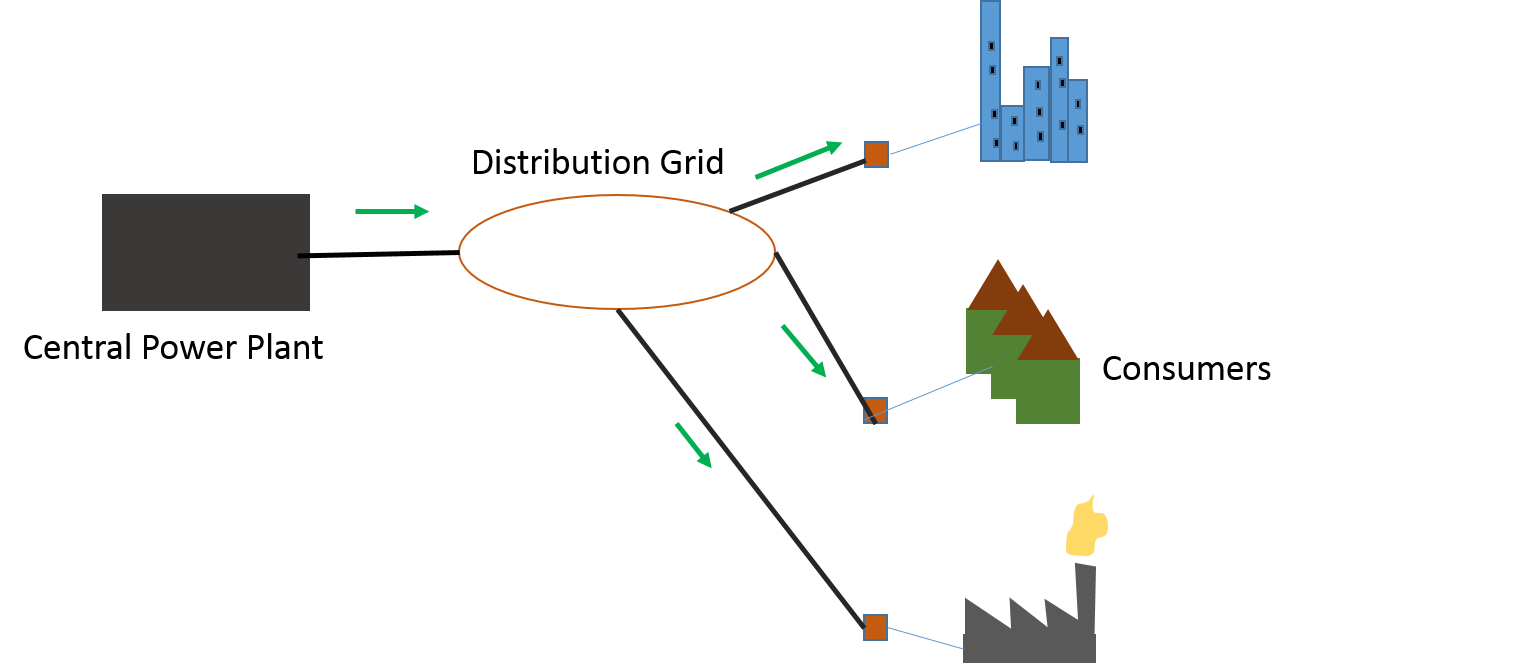
\includegraphics[width=\linewidth]{traditional.png}
  \caption{Traditional electricity generation and distribution system.}
  \label{fig:tradgrid}
\end{figure}

In contrast to the traditional electricity generation system, the Smart Grid (SG) is two-way \cite{fang2012smart}. Any node in the distribution grid can both consume and produce electricity to supply to the distribution grid. In Figure \ref{fig:smartgrid} a smart grid based electricity generation and distribution system are depicted. We can see that, in this system a flow toward the distribution system is possible. For example, renewable energy sources and household customers with solar energy production capabilities are pushing electricity to the power grid. The National Institute of Standards and Technology report \cite{fang2012smart} states that the SG could make the electricity generation and supply robust against generator or distribution node failure, promote the use renewable energy, widely and efficiently, reduce greenhouse gas emissions, reduce oil consumption by encouraging usage of electric vehicles, and give customers more freedom to choose among energy sources. Smart grids will encourage usage of electric vehicles since these vehicles have the ability to store power in a battery and transmit the power to the distribution grid if there is a need. Customers are showing strong motivation to use renewable energy as indicated by the statistics that 20\% of total energy is from the renewable sources which are second after coal 24\%. Consumers are using renewable energy due to economic reward and environmental concern. The major challenge with the usage of renewable energy as part of the supply is that it is uncertain \cite{richter2012transitioning}. This uncertainty causes problems for predicting how much energy the SG can produce in a future time slot. To manage the SG efficiently we will need effective methods to predict both energy production and load demand so they can be balanced in real time \cite{potter2009building}.

\begin{figure}[h]
  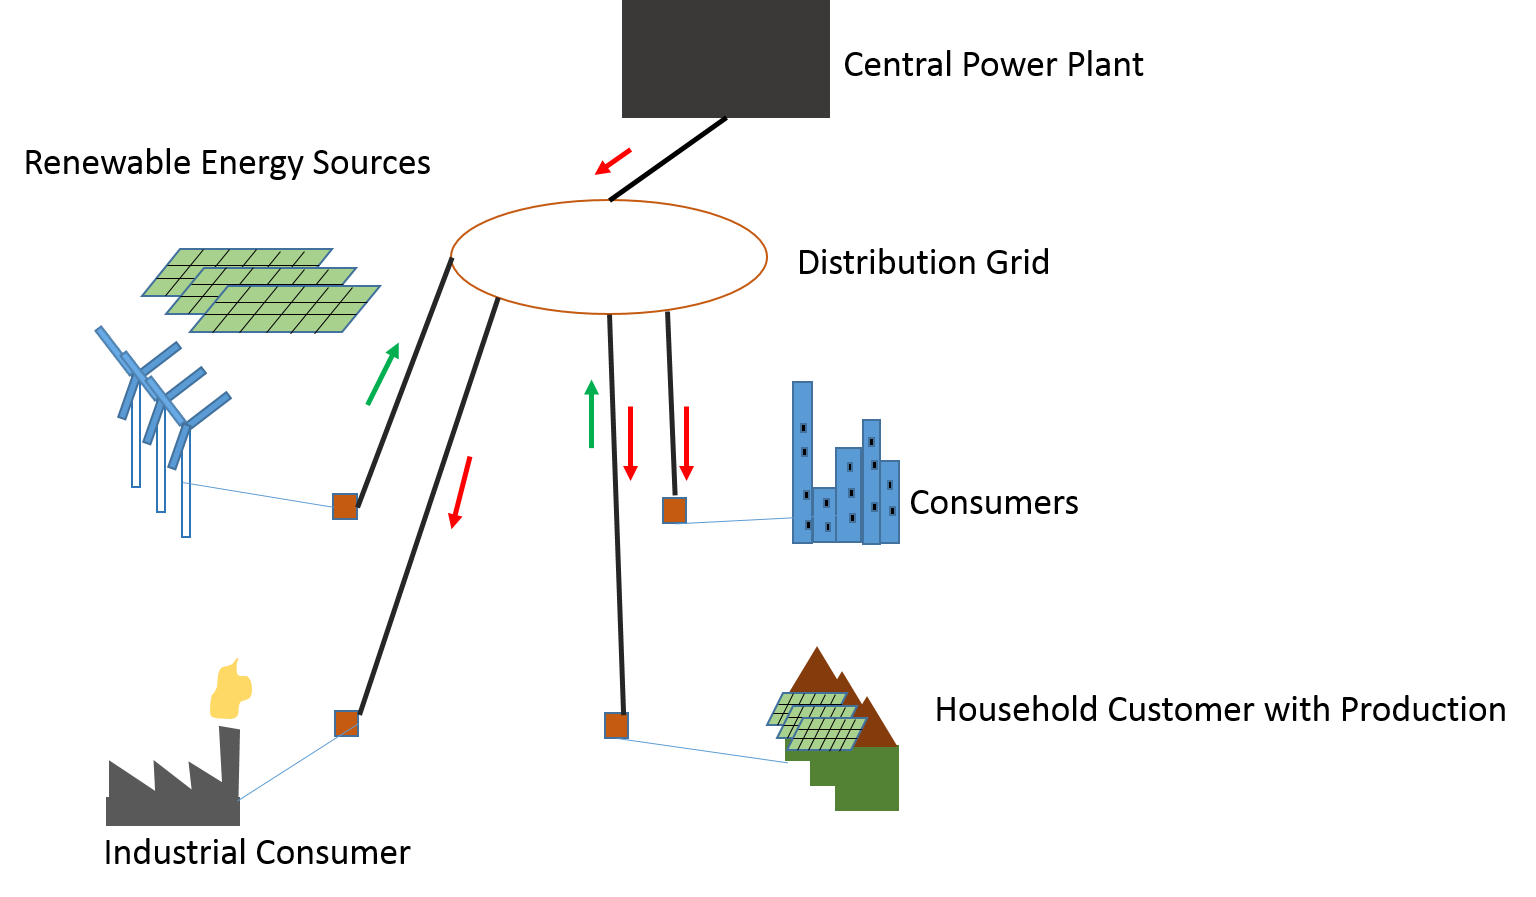
\includegraphics[width=\linewidth]{smart-grid.png}
  \caption{Smart grid based electricity generation and distribution system.}
  \label{fig:smartgrid}
\end{figure}

\section{The Power Trading Agent Competition}

The Power Trading Agent Competition (Power TAC) \cite{ketter2013power, ketter20162016}, is an international research competition based on a smart grid energy market and distribution system. The power TAC simulation models components including a wholesale market, electricity brokers, customers, a distribution utility and a weather service \cite{ketter20162016}. The brokers publish tariff plans for electricity consumers and producers. They buy electricity from the wholesale and balancing market to meet net customers demand. The system has realistic customer models and uses real weather data. Because of the realistic customer models present in the system, Power TAC can be used to do research on the customer electricity load demand. It is also useful because generating data is cheap in a computer simulation. The following sections give a brief explanation of each component of the Power TAC. Figure \ref{fig:simulation-environment}  shows a block diagram of the components of the powerTAC simulation environment.
%advantage 

\begin{figure}[!h]
  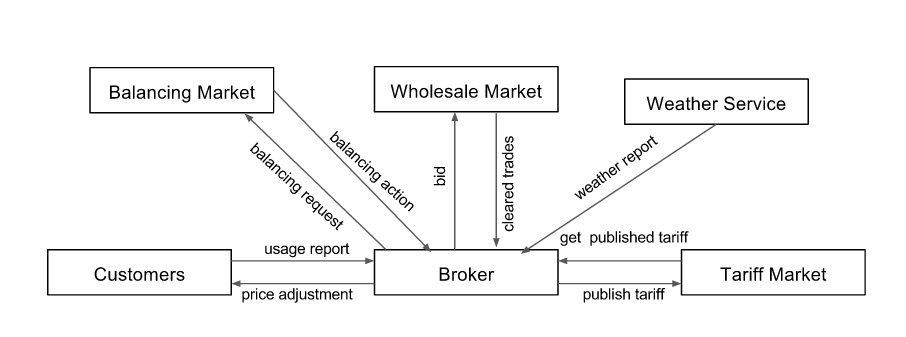
\includegraphics[width=\linewidth]{simulation-environment.png}
  \caption{PowerTAC simulation environment.}
  \label{fig:simulation-environment}
\end{figure}

\subsection{Markets and Distribution Utility}

There are three different types of markets in the Power TAC simulation, namely, the wholesale market, tariff market and balancing market. The wholesale market is the bidding place for buying or selling energy. Bulk energy producers and brokers take part in the wholesale market auction. Brokers can submit their bids for 24 future timeslots in the wholesale market by specifying the price they are prepared to pay. If the bid was successful, the broker receives the desired quantity by paying the money. At each time slot, the system notifies the broker about the wholesale market clearing prices. Brokers publish their tariff plans in the tariff market. A tariff holds information about the pricing of the energy. Customers, upon analyzing available tariffs, subscribe to the most suited tariff plan. The balancing market represents the market from where the broker can buy energy in case of imbalance. For example, if a broker has bought less amount of energy for a given timeslot and it finds it needs more energy then it can buy the necessary amount of energy from the balancing market. Usually, the balancing market transactions are more costly for brokers than the wholesale market.

The distribution utility has two main objectives. First, it supplies energy to the consumers from the wholesale market and from the renewable producers. Secondly, it works as a default broker that publishes default tariffs at the start of the game. This makes sure no customer is ever out of energy. Other brokers are supposed to publish more lucrative tariffs to attract customers.

\subsection{Brokers}

In the Power TAC game, participants implement a fully autonomous broker agent. A broker in the simulation competes with the other brokers by publishing competitive tariffs. The goal of a broker is to maximize its profit by buying electricity in a cheap price and selling the electricity in a profitable price. Here is the list of actions that a broker can take in Power TAC simulation:
\begin{itemize}  
\item At any hour of the simulation, a broker can publish a new tariff. Each tariff is targeted to a specific category of customers. The tariffs contain information about which category of customers it is targeted, the expiration date of the tariff, signing bonus, the penalty for early withdraw, and the rate of periodic payment. 
\item At any time, a broker can modify its published tariffs. It can adjust payment rates and withdraw penalty. The broker can also revoke a tariff that is not profitable.
\item To meet customer demand, a broker takes part in the electricity auction in the wholesale market. The wholesale market is the meeting place for bulk electricity sellers and brokers. The broker specifies how much electricity it needs, how much it is ready to pay for and at which time it needs the electricity. The broker can make asks or bid for next 24 hours. Based on the asks and bids from other brokers in the simulation, the broker's bid may or may not get cleared. 
\end{itemize}

At any moment in the simulation the brokers have the following information : 
\begin{itemize}  
\item Participating brokers in the simulation 
\item Information such as population, power types of the customers present in the simulation.
\item Initial electricity usage data of customers and initial clearing prices of the wholesale market.
\item Published tariffs in the simulation.
\item Information about tariff modification or revocation.
\item Wholesale market clearing prices for the last time slot.
\item Energy transaction information of subscribed customers.
\item Transaction in the balancing market.
\item Current bank balance for the agent.
\end{itemize}


\subsection{Customers}
A customer represents an entity that buys energy from or sells energy to the brokers. A customer tries to minimize its costs by subscribing to a broker that offers profitable tariff for the customer. The customers occasionally evaluate the tariffs present in the market and switch to a profitable tariff if necessary. Customers decide the outcome of a competition as the customers are the only consumers present in the system. A customer has the following attributes :
\begin{itemize}  
\item A unique name. 
\item Number of individuals the customer represents. This number can range from one to several thousand. 
\item A power type that specifies which category of customers (producer or consumer) the model falls into. Producer and consumer categories have several subcategories. In Power TAC the categories of the customers are consumption, interruptible consumption, thermal storage, wind production, solar production and electric vehicle. Each customer type has its distinctive behavior. 
\end{itemize}

A customer can take the following actions during a simulation - 
\begin{itemize}  
\item Evaluate available tariffs in tariff market.
\item Subscribe to or abandon a tariff. Customers try to maximize their economic gain so if there is a lucrative tariff in the market, a customer might try to subscribe to it.
\item Generate meter reading based on produced or consumed energy. The system then sends this meter reading to the broker it subscribed to. 
\item Customers with demand shifting capabilities can shift their demand to a favorable time slot.
\end{itemize}
 
Customer models and load forecasting problem will be described in more detail in Chapter \ref{customer-description}.

\subsection{Weather Service}
The weather service broadcasts weather forecast for future hours and a weather report for the current hour to the brokers. The weather report contains information such as wind speed, cloud cover, temperature, the day of week and month of week. Power TAC uses real weather data from the past to make the simulation more realistic. Brokers can use this information to forecast demand for the weather sensitive consumers. The weather information also makes it possible to forecast renewable energy production.



\section{Importance of Accurate Demand Forecasting in Power TAC}
A broker has to make bids and asks in the wholesale market. The amount of electricity it asks for depends on the demand forecast of its subscribed customers. If the broker fails to make an accurate demand forecast, it will not be able to ask for the proper amount of electricity. So it will end up asking more or less energy than the required amount in the wholesale market. In this case, the broker will have to buy energy from the balancing market at a higher price, or have to sell surplus electricity at a lower rate. As a result, it will face monetary losses. This unwanted scenario can be avoided through demand forecasting as accurate as possible. My thesis investigates ways to find a better demand forecasting mechanism.

\section{Main Research Questions}
The brokers in Power TAC get only 5 seconds of time to communicate with the server. Within the 5 seconds, it has to decide how much electricity the customers are going to use, decide on an ask with a profitable bid and make other decisions. It will be advantageous if there is a way to have a single forecasting model that gives the aggregated demand prediction for all customers in a single shot. So my first research question is: 
\begin{displayquote}
How effectively can we make a single demand forecasting model that make demand forecasting about all the customers in a single shot?
\end{displayquote}

As I solve the forecasting problem by training machine learning models, and the accuracy of the model will depend on which features I choose. If I can identify the most predictive features, the system will have less error. The second research question focuses on this problem:
\begin{displayquote}
What are the most relevant features for the demand forecasting model?
\end{displayquote}

Not all learning algorithms are suitable for a given scenario. I will be looking for learning algorithms that can be trained fast, that produces demand forecast as accurate as possible and makes predictions quickly. My third research question is:
\begin{displayquote}
Which learning algorithms are the most suitable for the Power TAC scenario?
\end{displayquote}

The system should be robust enough to be able to make demand predictions about a novel customer. My fourth research question is:
\begin{displayquote}
Can we develop an effective way to make a forecasting model trained on known customers and that can forecast the demand of a novel customer?
\end{displayquote}

I also need to see how the training set size impacts the accuracy of the forecasting model. If more training data the accuracy improves, I will try to gather as much data as possible until there are diminishing returns. My fifth research question is:
\begin{displayquote}
What is the impact of training set size on the accuracy of the prediction model?
\end{displayquote}
 
\section{Contribution}
In previous work on Power TAC, all the customers were treated the same. This work shows that different customers should be treated differently. I showed a demand prediction scheme for consumption type customer might not be suitable for interruptible consumption customers. This work proposes a method to make demand forecasting about a novel customer. During the training phase, known customers are grouped based on their weekly average electricity usage. Data of the same group are combined to make forecasting model for that group. A novel customer is assigned to one of the groups based on its weekly average electricity usage. The forecasting model of that group will be used to make forecasting about the new customer. This scheme produces better forecasting than a moving average baseline forecasting scheme. My work also found that there is little correlation with the accuracy of the system and the size of the training dataset. 

\section{Overview of the Thesis}
In the second chapter of the thesis I present related work on electricity demand forecasting. In chapter 3, I present information about the customers present in Power TAC. The information include customer types, their behaviors and descriptive statistics about them. In chapter 4, I present the work I did to answer the research questions and show the results. In chapter 5, I present the significance of the results and future work.


%%% Local Variables: 
%%% mode: latex
%%% TeX-master: "thesis"
%%% End: 
         % Chapter 2
% chap3.tex (Definitions and Theorem)

\chapter{Related Works}



In this chapter I will describe what other works has so far been done to predict customer's future energy demand.

%motivation for good prediction
Predicting customer's energy demand is important becasue failure to predict the demand accurately can cause monetary and environmental loss. Customer's with shifting load can use the energy produced by the renewable energy. Those customers can shift their load to a time where there is a high probablity of renewable energy production.

%Why are we using the powerTAC
Acting directly on the real environment can be risky. The powerTAC simulation system gives a low risk platform where the researcher's can build and test their works before deploying to real world. 

%types of load forecasting
There are different types of load forecasting namely short term load forecasting and long term load forecasting. Short term load forecasting deals with forecasting the customer's demand has the range of time couple of weeks. Long term load forecasting may forecast customer's demand over month or year \cite{cho1995customer}.

%TAC tex 13
TACTEX'13 won the PowerTAC competition in 2013. In a week a customer have 24 * 7 = 168 slots. TACTEX'13 the winner of PowerTAC competition 2013 kept track of average usage of 168 weekly slot for each customer. To predict a future time slot, their agent would look at at which weekly slot the future time slot would fall in. Then the agen uses that weekly slot's average usage as the prediciton of the future slot.

%talking about use of arima model
The ARIMA model uses both moving average and auto regression to forecast the demand. To make a forecast about a future time slot, the auto regression model uses some previously observed time slots values based on its degree. Moving average scheme would use the average of all the known time series data points to make a prediciton about a future time slot .Problem with univariate ARIMA model is that they don't take into account other variables that my affect the demand such as temperature. \cite{cho1995customer} attempted to forecast the energy demand for a region of Taiwan. They found temperature has effect on the energy usage of customers. To make prediction about the demand they used a transfer function that relates the daily temperature with energy usage along with the ARIMA model. This scheme resulted better than the univariate ARIMA model. They manually clustered the population in four categories such as commercial, office, residendial and industrial customers. 

%talk about influence of temperature
Intuitively weather variables such as temperature seem to have some effect on how much energy people use. Researchers have found that weather effect relies on the time duration the training data has. \cite{chen2004load} trained a SVM energy demand predictor that would predict energy demand of customers for the month January. The training data consited of every half hour's electricity demand from 1997 to 1998, average temperature from 1995 to 1998. They trained the predictor with only the portion of data that are related to the month January. They have found that within the month of January the temperature does not vary much and excluding the temperature from the feature set actually gives better prediction. Again, if energy demand is long term which means the window of prediciton is about a year, the temperature seems to have effect on the energy demand of the customers. \cite{hart2004weather} collected data of 18 months from households of a region of Australia. They collected the weather data from weather office and from self transplanted devices. They observed how the household customers use appliances based on the temperature. They came into conclusion that for that region, equilibrium point for energy is usage at temperature 0.25 degree celcius. If the temperature increases or decreases from this temperature, the electricity usage increases. They explained the behavior by stating as the temperature decreases, houses customers tend to use heaters and if the temperature rises they tend to use coolers more.

%talk about regional load forecasting
Regional load forecasting will enable us to know which regions need more energy. If we know which regions need more energy, we will know most suitable places to place electricity generator plants. \cite{hsu2003regional} worked on load forecasting based on region. They diivided electricity usage of Taiwan in 4 areas. For each region, they collected GDP,  population, highest temperature and aggregated load. After that, they trained Artificial Neural Network model for each region. For baseline, they trained linear regression model for each region. The result showed that, the ANN based load forecasting methods performed better than the linear regression  methods. 

%talk about clustering for load forecasting
\cite{mcloughlin2015clustering} have used clustering method to forecast customer's future electricity demand. They collected data from more than 4000 household customers in Ireland for about 6 months. Collected data included electrecticity usage at 30 minutes interval, appliances used in the home and different socio-economic information about the people living in a particular house. They clustered each days usage which they call load profiles. A customer's daily usage then can be assigned to one of those load profiles. The customer is then charactersized by the the mostly used load profile. The authors then train a linear regression classifier that was built upon the socio-economic information of a the customers, types of appliances used in the house and the description of the house to figure out the common load profile of the given household. The predicted load profile of the customer received from the linear regression model will be used to predict the demand of the customer for a given day.
 

%talk about influence of behavior for modeling customers
\cite{lampropoulos2010methodology} the authors proposed a methodology to model electric car user cusotmer's demand. They uses data of electric car users of Netherlands from 2000 to 2007. The data included purpose and starting time of each drive, duration of the drive and the time the driver spent at the purpose destination and when the time when the driver returned home. From this data, the authors found usually the drivers would recharge their car at around hours 17:00 to 19:00. So the electricity generators may find this time a peak demand time due to the added energy demand of the electric vehicle customers. 

%talk about choosing similar days to forecast demand
\cite{liu2006accurate} the authors observed load of certain hour of a certain day is highly correlated with load of some certain days before that day. On the basis of the observation, they would take ten most similar looking days electricity usage and feed it to an ANN to make forecast of the day. The authors found the other variables that may affect the load such as temperature, humidity may change so swiftly that inclusion of them may reduce the accuracy of the predictor. So they excluded all the social, environmental variables from their model of prediction.

%expert systems for load forecasting
The authors in ref \cite{rahman1988expert} have proposed an expert system based load forecasting method for the region Virgina. The expert system would forecast load of upcoming 24 hours. They observed the variables that are likely to affect the load. They came up with variables such as temperature, load of previous hour, season and day of week have strong correlation with the observed load. They implemented a computer program that mimicked how a human operator makes load forecast based on the independent variables. For a specific region's weather condition, their method worked well and required limited amount of historical data.

%machine learning based approaches
\cite{parra2013initial} the authors used varios machine learning techniques to make 24 hour ahead load forecast. They found that hour of week, weather related features such as temperature cloud cover were influential to the electricity load. They created one machine learnign forecasting module for each customers by extracting relevant features of the customers. The forecasting modules performed well for the customers that shows regularity in their energy consumption behavior. For the customers with load shifting capabilities to their favored hour, the scheme did no perform well.

%inlfluence of the variables
In the survey article \cite{hahn2009electric}, the authors reported variables that are likely to affect the electricity load. According to them, univariate models are adequate if the load forecast is upto 6 hours ahead. If the target is to make load forecast with larger window, including more available variables such as weather related information and day of week's information can be helpful. There are three types of cycle in the load curve, daily, weekly and seasonal. At a certain time of a day load is usually higher or lower. Again, in a week, there are two visible pattern in weekend and weekdays. The days that are neighbor to the weekend such as Friday and Monday are also get influenced by the weekend days. The season and area under consideration also strong correlation with the electricity load.         % Chapter 3 
% chap4.tex (Customer Description)

\chapter{Customer Description} 

In this chapter, I will describe the customers present in the Power TAC simulation system and some statistics about their attributes.

\section{Customer Categories}


In Power TAC simulation, a customer can be electricity consumer or producer based on the power type it has. A customer evaluates the tariff plans targetted for its power type and can look for the tariff that gives it maximum monetary benefit. There are several types of customers in the Power TAC simulation such as consumption, interruptible consumption, thermal storage, solar production, wind production and electric vehicle. Each power type has its own characterstics. For example, interruptile consumption customers can shift their electricity demand to some off peak hour, the solar production customers can produce energy based on the weather condition. As opposed to previous methods on demand forecasting, I argue that each category of customers based on the power type should be treated differently. One load forecasting method can be suitable for a category of customers while it may be unsuitable for other categories because each category behaves differently. I describe the characterstics of the customers below -

\begin{itemize}
\item \textbf{Consumption: } A customer with power type consumption are the most common customers. They use the energy when they need it. They cannot shift their demand to a future timeslot. Usually, they have a regular electricity usage pattern. Often, they show a similar pattern for weekdays. Often, they have similar kind of usage pattern for the weekends. 



\item \textbf{Interruptible Consumption: }
Interruptible customers are smart enough to shift their energy demand in a timeslot where they can buy electricity at a reduced price. Because of this shifting capability, they don't show a regular usage pattern as the consumption customers do. 

\item \textbf{Thermal Storage: }
Thermal storage customers show a weekly pattern in their electricity usage. Also, during a day, their electricity usage in a day depends  much on the energy they used in the last timeslot. 


\item \textbf{Solar Production}
The solar energy production customer's energy production depends on the cloud cover. They are highly likely to produce energy during the day time.

\item\textbf{Wind Production} Wind production customers generate energy from the wind.
\item \textbf{Electric Vehicle} An electric vehicle customer represents one electric vehicle. Their usage of energy is quite irregular and hard to predict. \\
\end{itemize}

 To discuss the behavior of different power typed ustomers, a representative customer was chosen from each type. The table \ref{table:repCust} shows the customer chosen to discuss -

\begin{table}
\centering
\begin{tabular}{ |c|c| } 
\hline
Power Type & Customer Name \\
\hline
Consumption & downtown offices \\ 
Interruptible Consumption & village 1 ns \\ 
Thermal Storage & sf2 \\ 
Solar Production & sunnyHill \\ 
Wind Production & windmill 1 \\ 
Electric Vehicle & high income 1 \\ 
\hline
\end{tabular}
\caption{Representative customer from each power type}
\label{table:repCust}
\end{table}

Before diving into the problem of solving forecasting methods, I found it useful to take a look at how the customers of differnet power types behave. A log extractor program extracts all the energy consumption and production by all the customer on all the timeslot. At the end of the game, it makes a report on normalized usage of all the customers in all the week slots. Normalized values are useful because even if the amount of energy usage among the customers vary, the pattern of usage can be captured through it and normalized usages of different customers can be plotted in the same graph. The figures \ref{fig:daily1} to \ref{fig:daily3}, shows normalized electricity demand or supply of Mondays. 0 in the x axis means hour 12:00 am. From the figures \ref{fig:daily1} to \ref{fig:daily3}, it is clear that some customer's electricity usage is higly correlated with time of the hour of the day. The customers of type consumption and solar energy can be example of these types. The other customer type demands did not seem to have correlation with an hour of a day. In both consumption and solar energy customers the consumption or production curve grew smoothly till it reached a peak point. After the reaching the peak, the production or consumption reduced smoothly. The customers with types interruptible consumption, wind production, thermal storage and electric vehicle had irregular demand/supply pattern. 

In figure \ref{fig:weekly1} to \ref{fig:weekly3}, normalized electricity usages during the week are shown. Hour 0 to 23 represents all the hours of Monday from 12:00 am to 11:00 pm. It appears that, the electricity demand for consumption customer, interruptible consumption, thermal storage had repeatative demand pattern everyday. The  solar energy production customer showed repeatative production pattern. Moreover some customers such as the consumption type and the thermal storage type showed different pattern during the weekend. During the weekend they usually had lower energy demand than the weekdays. In the case of electric vehicle and wind energy production customers the demand/supply patterns were not regular. From these observations, it can be assumed that the consumption customer and the solar energy type customers can be forecasted with the most accuracy. Due to the irregular patterns of other customers, it will be harder to make accurate demand forecast about them.
 
% figure start
\begin{figure}
\centering
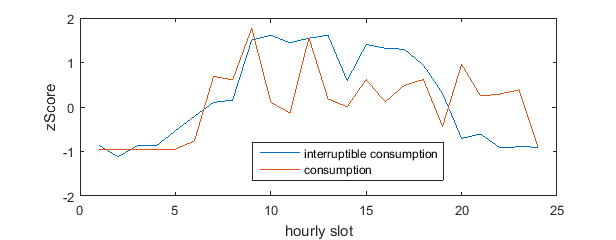
\includegraphics[scale=0.9]{daily1.png}
\caption{energy usage z Score over Monday}
\label{fig:daily1}
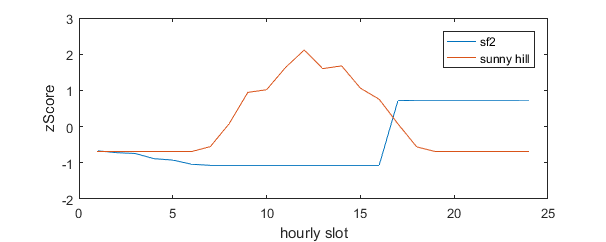
\includegraphics[scale=0.9]{daily2.png}
\caption{energy usage z Score over Monday}
\label{fig:daily2}
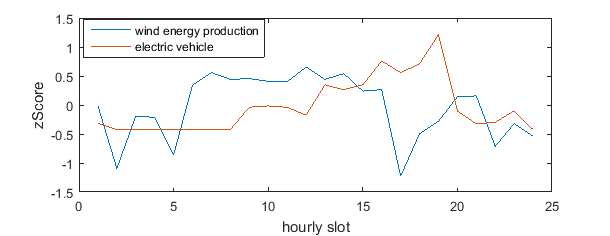
\includegraphics[scale=0.9]{daily3.png}
\caption{energy usage z Score over Monday}
\label{fig:daily3}
\end{figure}

\begin{figure}
\centering
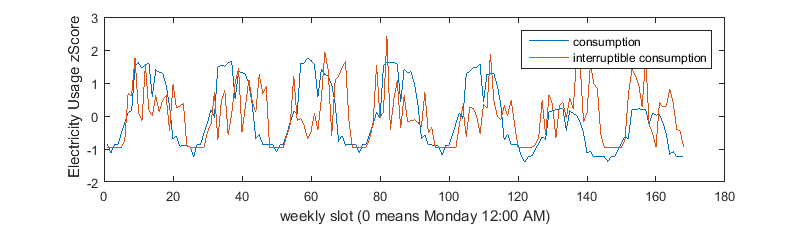
\includegraphics[scale=0.85]{weekly1.png}
\caption{energy usage z Score over week}
\label{fig:weekly1}
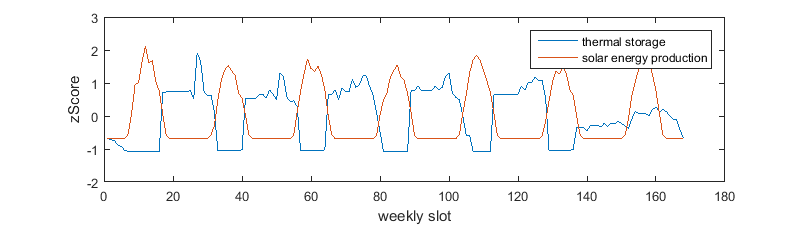
\includegraphics[scale=0.85]{weekly2.png}
\caption{energy usage z Score over week}
\label{fig:weekly2}
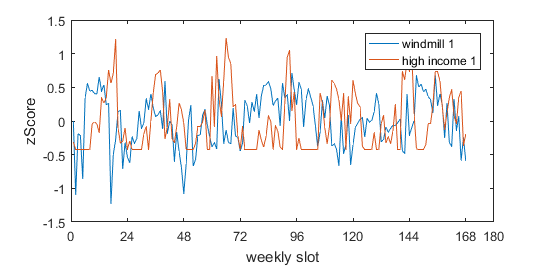
\includegraphics[scale=0.85]{weekly3.png}
\caption{energy usage z Score over week}
\label{fig:weekly3}
\end{figure}

%figure end

\section{Statistics}
In this section, I present some statistics on the customers available in the system. 

\begin{itemize}
\item \textbf{Customer Vs PowerType}

The figure \ref{fig:cust-pt} shows number of customers in each power type for a typical Power TAC simulation game. The electric vehicle power type has the most number of customers. This is because the electric vehicle represents a population of size 1. Consumption and interruptible consumption power type customers follow the electric vehicle power type customers in terms of number of customers. 

\item \textbf{Population Vs PowerType}
From figure \ref{fig:pop-pt} by far the powertype of consumption has the most number of population. Some customers can represent thousands of individuals. For this reason, even though there are only a few numbers of consumption and solar energy customers, they can represent a population of size several thousands. 

\item \textbf{Total Energy Consumed Vs PowerType}
The figure \ref{fig:energy-pt} and \ref{fig:energy-shares} show the contribution in energy transaction by different power type customers in a typical Power TAC simulation. From the figures, we can see that the consumption type customers are responsible for the most amount of energy transaction (more than 60\%). After the consumption type customers, the interruptible consumption type customers trade 18\% of total traded energy. The solar production customers caused the 11\% of total energy transaction. Undoubtedly, a successful broker needs to forecast the consumption type customer with prime importance because of the bulk of energy they transact. Due to this fact, I concentrated mostly on forecasting about consumption type customers' demand.


\begin{figure}
\centering
\begin{minipage}{.5\textwidth}
  \centering
  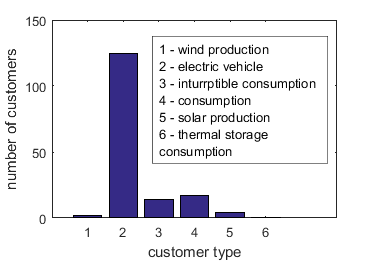
\includegraphics[width=\linewidth]{4-customer-vs-powertype.jpg}
  \caption{Number of customers vs Powertype.}
  \label{fig:cust-pt}
\end{minipage}%
\begin{minipage}{.5\textwidth}
  \centering
  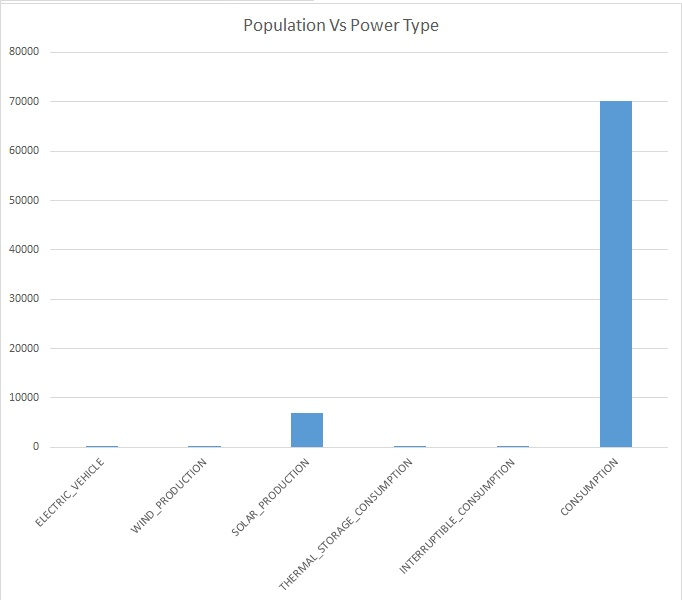
\includegraphics[width=\linewidth]{2-population-vs-powertype.jpg}
  \caption{Population vs Powertype}
  \label{fig:pop-pt}
\end{minipage}

\centering
\begin{minipage}{.5\textwidth}
  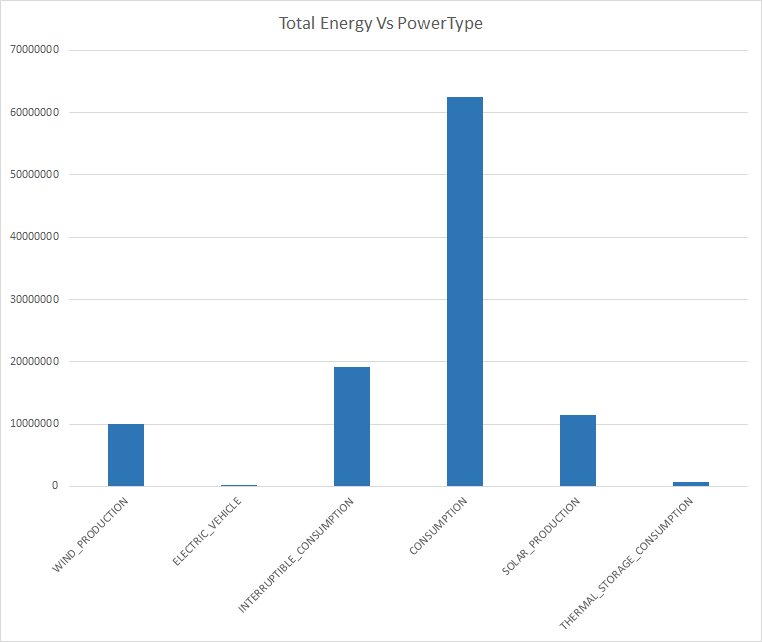
\includegraphics[width=\linewidth]{3-energy-vs-powertype.png}
  \caption{Energy vs PowerType.}
  \label{fig:energy-pt}
\end{minipage}%
\begin{minipage}{.5\textwidth}
  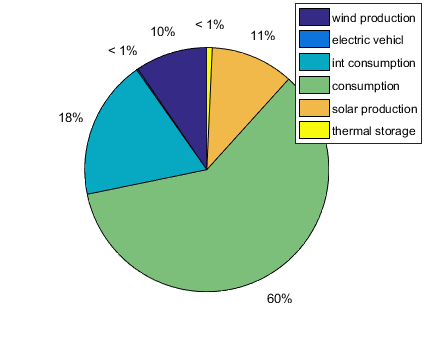
\includegraphics[width=\linewidth]{pie-energy-share.png}
  \caption{Energy share for each power type.}
  \label{fig:energy-shares}
\end{minipage}

\end{figure}

\end{itemize}
         % Chapter 4 customer description 
% chap5.tex (Methodology and Result)

\chapter{Methodology and Results}

In this chapter, I describe the methodologies I followed to find answers to the research questions I have described in Chapter 1.


\section{Learning Algorithms, Training and Test Set}
I have tried several learning algorithms that are available in Weka \cite{witten2005data}. I was looking for learning algorithms that can be trained as quickly as possible with a large amount of data and with limited computing resources. The learning algorithm also has to produce a lower error rate and fast output during the time of competition. I have found that M5P, M5RULES, REP TREE, LINEAR REGRESSION \cite{witten2005data} met my requirements. For training the models, I have used 10 game log files. Each log files contain about 10,000 training instances. A training instance contains the values of independent and dependent variables values. In the case of my thesis, example of independent variables would be temperature, cloud cover etc. and the dependent variable would be actual electricity usage of customers. Training time was getting more than 48 hours when I was using more than 10 log files. I separated 5  log files randomly from set of available game log files to use as a test set. The log files included in the test set were not used in training.

\section{The Baseline Electricity Forecasting Mechanism}
The first baseline energy forecasting mechanism is the default prediction mechanism provided by the Power TAC system. It exploits the fact that usage of a timeslot of a customer in a specific date is highly correlated with the day of a week and hour of a day. To make a prediction it stores the average energy usage of an hour of a week. So, for each customer, it uses $24*7 = 168$ values to remember average usages. As soon as it is informed of the new usage information of an hour of a week, it updates the old average using the Algorithm \ref{alg:updateAvgMovingAvg}. To make demand forecasts about a customer it uses Algorithm \ref{alg:predictAvgMovingAvg}.

\begin{algorithm}
\caption{Update average usage for $customer_i$ for day d and timeslot t, $newUsage$}
\begin{algorithmic} [1]
\STATE avgUsage = get average usage of $customer_i$ at day d and time slot t
\STATE $avgUsage = 0.7 * avgUsage + 0.3 * newUsage$
\end{algorithmic}
\label{alg:updateAvgMovingAvg}
\end{algorithm}

\begin{algorithm}
\caption{forecast usage for day d and timeslot t for $customer_i$}
\begin{algorithmic} [1]
\STATE avgUsage = get average usage of $customer_i$ at day d and time slot t 
\STATE return $avgUsage$
\end{algorithmic}
 \label{alg:predictAvgMovingAvg}
\end{algorithm}

\section{Feature Extraction}
	All the activities that occurred in a game can be found in a game log.  Activities such as buying or selling electricity occur during a time slot. At the beginning of a time slot, the system notifies the broker that a new time slot is about to begin. The system also notifies the brokers with weather forecast about the future time slots. As a time slot ends, the broker receives information about its customer's energy usage which is called tariff transaction report. From game log file, a feature extractor program can extract features related to customer time related information, electricity usage and weather variables. By keeping the previous electricity usage  history for each customer, it is also possible to generate useful statistics such as mean and standard deviation usage for each hour of a week day. Algorithm \ref{alg:ttxHandle} specifies how the extraction program retrieves the necessary information from the tariff transaction report. As the broker gets notification of the beginning of a new time slot, the extraction program has all the information related to energy usage and weather data of the previous time slot. 
%feature extraction
\begin{algorithm}[!h]
\caption{extract information from transactionReport sent to broker after each time slot through TariffTransactionHandler call back method}
\begin{algorithmic} [1]
\STATE timeSlot = get time slot from transactionReport
\STATE customerName = get customer name from transactionReport
\STATE energyUsed = get energy used from trom transactionReport
\STATE addUsage(customerName, timeSlot, energyUsed)
\end{algorithmic}
 \label{alg:ttxHandle}
\end{algorithm}

%write extracted features
\begin{algorithm} [!h]
\caption{write extracted data after timeSlot update message received from TimeSlotUpdateHandler call back method}
\begin{algorithmic} [1]
\STATE knownTimeSlot = timeSlot - 1
\FOR{each customer}
\STATE day = get day of knownTimeSlot
\STATE hour = get hour of knownTimeSlot
\STATE statisticalData = get statistics of the customer of day and hour
\STATE weatherData = get weather data of knownTimeSlot
\STATE trueUsage = get true usage of customer in knownTimeSlot
\STATE trainingInstance = create training instance by combining statistical data, weather data and true usage 
\STATE writeToFile(trainingInstance)
\ENDFOR
\end{algorithmic}
\label{alg:writeSlotInfo}
\end{algorithm}

\section{Single Demand Predictor}
The single demand predictor is designed to make a single aggregated load demand forecast for all the customer in a single shot. It is trained with 54 features. The features included time-related features such as day of week, hour of day, month of year; weather-related features such as cloud cover, wind speed, temperature; historical data such as past 24 slot's electricity usage, last week's electricity usage and statistical features such as average and standard deviation of the weekly slot. Algorithm \ref{alg:bestSingle} shows how a single prediction model is created. At first, features extracted from all types of customers are combined to make training set. Several classifiers are then trained based on the training set using 10 fold cross validation \ref{witten2005data}. It can be seen that the training set had information about all the customers of all types discussed in Chapter 3. For this scheme the baseline predictor produced on average 70\% root relative percentage error \ref{witten2005data}. And for all learning algorithms, the error rate was more than 80\%. The reason behind this poor perfomance is irregularity in training data. As we saw earlier, not all customers have regularity in their electricity usage pattern. As I have aggregated information about all the customers, which included irregularity, the training model is not able to generalize knowledge from the training set properly using the features and data available. 



%find best performing single prediction model
%find best classifier for individual customers
\begin{algorithm}[!h]
\caption{find a single best classifier}
\begin{algorithmic} [1]
\STATE combine all slot based training instance of all the customers
\STATE train available classifiers on the combined data using 10 fold cross validation
\STATE choose the classifier with minimum error
\STATE save the classifier for making prediction about all the customers
\end{algorithmic}
\label{alg:bestSingle}
\end{algorithm}

\section{Individual Demand Predictor}

From the experience of a single demand predictor, I included only information about consumption customer data in training set and excluded information about interruptible consumption, thermal storage and electric vehicles power type customers. Also, this time I reduced the number of features using Weka's attribute selection algorithm \cite{witten2005data}. Out of 54 features, only 5 were choosen. The features selected were temperature, wind speed, cloud cover, average of the weekly hour slot, standard deviation of the weekly hour slot. Features extracted for each customer served as a separate training data set. I trained an individual predictor model for each customer model. In general, if there are \textit{n} customers in the system, we will need \textit{n} electricity demand predictors, each trained on the data of a single customer. I went further by checking different machine learning algorithms such as M5Tree \cite{witten2005data}, Linear Regression \cite{witten2005data}, M5P rules \cite{witten2005data} and REP tree \cite{witten2005data} for each customer and picking the best performing one for each customer. The process of finding best prediction model for each customer is shown in Algorithm \ref{alg:bestClassifierForCluster}. Each prediction model will make an electricity load demand prediction for each customer. The broker can calculate the total electricity demand by summing over all the predictions.

\begin{algorithm}[!h]
\caption{find best classifiers created for each individual customer}
\begin{algorithmic} [1]
\FOR{each customer}
    \STATE combine all slot based training instance of the customer
    \STATE train available classifiers on the combined data using 10 fold cross validation
    \STATE choose the classifier with minimum error
    \STATE save the classifier for making prediction about the customer
\ENDFOR 
\end{algorithmic}
\label{alg:bestClassifierIndiv}
\end{algorithm}


\section{Cluster Based Demand Predictor}
One problem with the individual demand predictor is that this system has a demand prediction model for each known customer. So, it cannot make demand forecasts for a novel customer. This is a serious problem because during a competition the system may introduce a new customer or change the name of a customer. In those cases the individual demand prediction mechanism becomes unreliable. To mitigate this issue, I propose a solution that groups similar customers based on their weekly average usage pattern. The Figures \ref{fig:toy-clust-1} and \ref{fig:toy-clust-2} depicts the proposed method. Figure \ref{fig:toy-clust-1} shows that when clustering is applied on the weekly average usage data of customers, the customers are grouped in different clusters. Figure \ref{fig:toy-clust-2} shows that once the clustering is done, training instances related to the members of a cluster is combined to train classifier for that cluster. At runtime, a customer will be grouped in a cluster based on its weekly usage. Once the program knows the cluster assigned to a customer, the program will load the corresponding classifier to make electricity demand forecasts about the customers.

\begin{figure}[h!]
  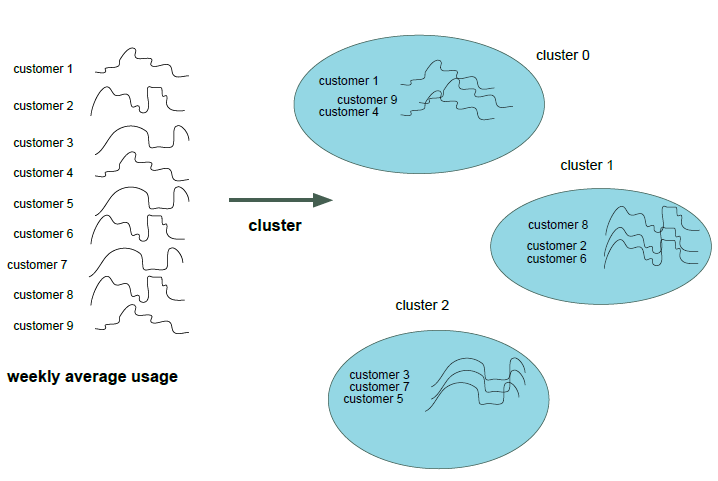
\includegraphics[width=\linewidth]{cluster-toy-1.png}
  \caption{Clustering customers based on weekly average usage. }
  \label{fig:toy-clust-1}
\end{figure}

\begin{figure}[h!]
  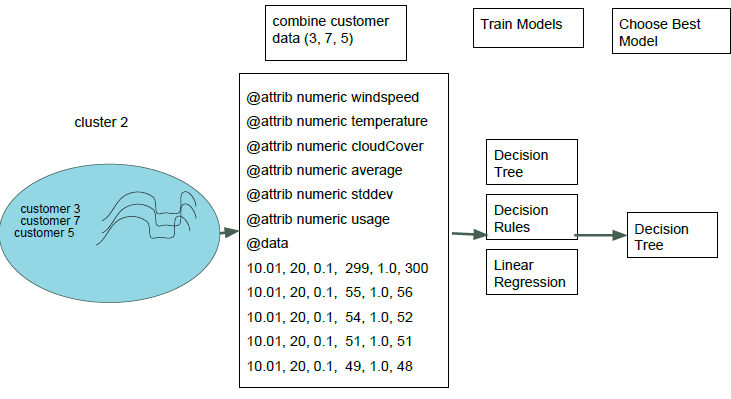
\includegraphics[width=\linewidth]{cluster-toy-2.png}
  \caption{Training prediction classifier for a cluster.}
  \label{fig:toy-clust-2}
\end{figure}

Algorithm \ref{alg:writeWeeklyAvg} shows the procedure for extracting average electricity usage of each hour of a week. Next, all the average weekly usages are combined together to make training set for the clustering algorithm. I have used k-means \cite{witten2005data} clustering algorithm to cluster the  training set. I have trained clusters of sizes 1 to 18. Algorithm \ref{alg:makeCluster} describes the procedure for making clusters from the training instances. Once a k-means of cluster size k is made, a program groups the hourly usages of the customers in the same cluster and combines them to make training set for  machine learning classifier. This training set is used to train a  linear regression classifier. Algorithm \ref{alg:errorOfCluster} describes how the cluster-based predictor's performance was evaluated. I fixed the optimal number of clusters from two observations. First, I used Expectation Maximizaion (EM) algorithm to see how many clusters might be present in the data. If number of clusters are unknown, EM algorithm can tell how many clusters are there. Secondly, I noticed the prediction error produced for each cluster of size k in kmeans clustering algoirhtm and observed for what size of cluster the error is minimum. The result is described in Section \ref{results}. Once the number of the clusters was fixed, a program creates several machine learning predictors to see which one performs best for a given cluster. The machine learning classifiers that were tried out are Linear Regression \cite{witten2005data}, M5P rules \cite{witten2005data}, M5 Tree\cite{witten2005data}, REP tree\cite{witten2005data}. 

\begin{algorithm} [!h]
\caption{write average electricity usage of the customers of each hour of the week}
\begin{algorithmic} [1]
\REQUIRE information of all timeslots has been received
\FOR{each customer}
    \STATE trainingInstance = create empty training instance
    \FOR{each day of week}
        \FOR{each hour of day}
            \STATE averageUsage = get average usage of day and hour of customer
            \STATE append averageUsage to the trainingInstance
        \ENDFOR
    \ENDFOR
    \STATE writeToAvgUsageFile(trainingInstance)
\ENDFOR
\end{algorithmic}
\label{alg:writeWeeklyAvg}
\end{algorithm}

%make cluster

\begin{algorithm}
\caption{create kmeans cluster of size k from weekly usage training instance file}
\begin{algorithmic} [1]
\STATE data = load weekly average usage file
\STATE kmeansCluster = build kmeans cluster of size k based on data
\STATE save kmeansCluster
\end{algorithmic}
\label{alg:makeCluster}
\end{algorithm}

%find size of k
\begin{algorithm}[!h]
\caption{find error of kmeans clusters of different size}
\begin{algorithmic} [1]

\FOR{each cluster size k}
    \STATE get the kMeansCluster of size k
    \FOR{cluster in KMeansCluster}
        \STATE combine slot based training instances of that cluster
        \STATE train linear regression classifier based on the combined data
        \STATE save the classifier for cluster
    \ENDFOR
\ENDFOR

\FOR{each training instance}
    \STATE compute error of the instance using each kMeansCluster
\ENDFOR
\end{algorithmic}
\label{alg:errorOfCluster}
\end{algorithm}

%find best classifier for cluster of size k
\begin{algorithm} [!h]
\caption{find best classifiers of each cluster of kmeans cluster of size k}
\begin{algorithmic} [1]
\FOR{each cluster in kMeansCluster}
    \STATE combine slot based data of the all the customers in cluster
    \STATE train available classifiers on the combined data using 10 fold cross validation
    \STATE choose the classifier with minimum error
    \STATE save the classifier for making demand forecasting for cluster
\ENDFOR 
\end{algorithmic}
\label{alg:bestClassifierForCluster}
\end{algorithm}

\section{Testing Performance}
Algorithm \ref{alg:performanceEval} shows how the accuracy of each prediction model was tested. Each instance of the test set was tested against each demand prediction scheme. The mean absolute percentage error (MAPE) \ref{witten2005data} was calculated for each scheme. Algorithm \ref{alg:errorCalculation} shows the algorithm for computing error.
 
%Testing
\begin{algorithm}
\caption{performance evalulation of each method}
\begin{algorithmic} [1]
\FOR{each test instance}
    \STATE classify the test instance using moving average usage \textbf{[algorithm \ref{alg:predictAvgMovingAvg}]}
    \STATE classify the test instance using individual prediction mechanism
    \STATE classify the test instance using cluster based predictor
    \STATE calculate and accumulate errors of each mechanism \textbf{[algorithm\ref{alg:errorCalculation}]}
    \STATE update moving average baseline predictor based on the information from the test instance \textbf{[algorithm \ref{alg:updateAvgMovingAvg}]}
\ENDFOR 
\STATE find average error from the accumulated errors for each forecasting mechanism
\end{algorithmic}
\label{alg:performanceEval}
\end{algorithm}
%calculate error
\begin{algorithm} [!h]
\caption{calculate error from the predicted value and the true value}
\begin{algorithmic} [1]
\STATE absoluteError = abs(predictedValue - trueValue)
\STATE relativeAbsoluteError = (absoluteError / trueValue ) * 100 \%
\end{algorithmic}
\label{alg:errorCalculation}
\end{algorithm}

\section{Experimental Results}

The following subsections describe the results at each stage of the experiments. The stages are 1) finding optimal number of clusters. 2) Once the number of clusters has been fixed, a different classifier needs to be made for each cluster to see which one makes the best forecast for a particular cluster. 3) After that, the baseline predictor that needs a classifier for each customer needs to be trained. At this point, for each customer several classifier has been tried out to see which classifier makes best demand forecast about that customer. 4) Finally, the proposed mechanism is tested against the two baseline demand forecasting methods.

\section{Finding Individual Predictor for Each Customer}
Based on the data from each of the customers, the four types of classifiers described previously were tested. For each customer, the Table \ref{table:1} shows the best performing classifier for each customer. 

\begin{table}[h!]
\centering
\caption{Best individual predictor for each customer}
\begin{tabular}{|c| c|} 
 \hline
 Customer Name & Best Predictor Type \\ [0.5ex] 
 \hline
BrooksideHomes &	M5P \\
CentervilleHomes &	M5P \\
DowntownOffices &	M5P \\
EastsideOffices &	M5P \\
OfficeComplex 1 NS Base &	LinearRegression \\
OfficeComplex 1 SS Base &	LinearRegression \\
OfficeComplex 2 NS Base &	LinearRegression \\
OfficeComplex 2 SS Base &	LinearRegression \\
Village 1 NS Base &	M5P \\
Village 1 RaS Base &	LinearRegression \\
Village 1 ReS Base &	M5P \\
Village 1 SS Base &	M5P \\
Village 2 NS Base &	LinearRegression \\
Village 2 RaS Base &	M5P \\
Village 2 ReS Base &	M5P \\
Village 2 SS Base &	M5P \\
MedicalCenter@1	& M5P \\ [1ex] 
 \hline
\end{tabular}
\label{table:1}
\end{table}

The figure \ref{fig:indiv-cutomer-best-predictor-error} shows error percentage of each of the predictors type for each of the customer types.

\begin{figure}[h!]
  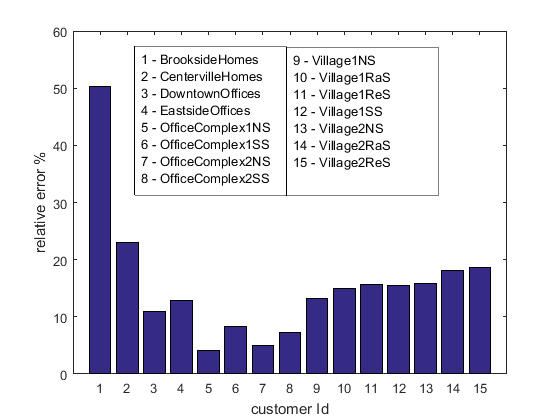
\includegraphics{relativeErrorIndivPredictor.png}
  \caption{Performance of the best classifier for each customer type. Customer Medical center was excluded as it was showing huge error. }
  \label{fig:indiv-cutomer-best-predictor-error}
\end{figure}

%%%%%%%%%%%%%%%%%

\subsection{Finding the optimal number of clusters} \label{results}

First, I segmented the customer using KMeans clustering algorithm with cluster sizes from 1 to 18. I choose the number 18 because there are 17 consumption type customers in Power TAC. In worst case, each customer may be different and there will be 17 clusters. For kMeans Eucleadian Distance \cite{witten2005data} was used for similarity metric, max number of iteration \cite{witten2005data} was set to 500. For KMeans with size k, we will have k clusters. For each of the k clusters, I had a linear regression predictor. I observed the relative percentage error and absolute average the above cluster sizes. Figure \ref{fig:cluster-error} shows the cluster size vs MAPE. It shows that after cluster of size 4, the size of the cluster does not have a big impact on the prediction performance. The EM algorithm reports that there are 4 clusters present in the data when max iteration parameter \cite{witten2005data} was set to 100, minimum standard deviation parameter \cite{witten2005data} was set to 1.0E-06 and num clusters parameter \cite{witten2005data} was set to -1. To keep things simple, I have decided to choose Kmeans cluster of size 4.  When k = 4 was chosen, the Table \ref{table:clusterAss} shows the cluster assignment for each customer. The Table \ref{table:clusterAss} shows that, cluster 0 held most of the offices, cluster 2 held most of the village types, cluster 3 held the medical center, cluster 1 held large housing such as brooksidehomes, centerville homes and large offices such as downtown offices and centerville offices. This observation suggests that the office, village, large corporation customers have similar kind of electricity usage pattern in Power TAC.

\begin{figure}[h!]
  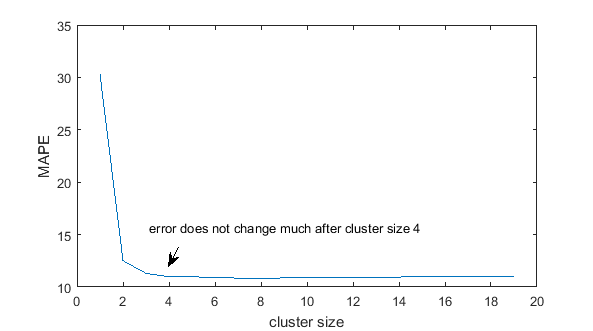
\includegraphics{cluster-error.png}
  \caption{Kmeans cluster size vs MAPE. }
  \label{fig:cluster-error}
\end{figure}

\begin{table}[h!]
\centering
\caption{Assigned cluster for each customer}
\begin{tabular}{|c| c|} 
 \hline
 Customer Name & Assigned Cluster Number \\ [0.5ex] 
 \hline
BrooksideHomes &	0 \\
CentervilleHomes & 0 \\
DowntownOffices & 1	\\
EastsideOffices &	1 \\
OfficeComplex 1 NS Base &	0 \\
OfficeComplex 1 SS Base &	0 \\
OfficeComplex 2 NS Base &	0 \\
OfficeComplex 2 SS Base &	0 \\
Village 1 NS Base &	2 \\
Village 1 RaS Base &	2 \\
Village 1 ReS Base &	2 \\
Village 1 SS Base &	2 \\
Village 2 NS Base &	2 \\
Village 2 RaS Base &	2 \\
Village 2 ReS Base &	2 \\
Village 2 SS Base &	2 \\
MedicalCenter@1	& 3 \\ [1ex] 
 \hline
\end{tabular}
\label{table:clusterAss}
\end{table}

\subsection {Finding the best predictor for each cluster}
Once the features are extracted, I have tested  M5Tree, Linear Regression, M5P rules and REP tree machine learning classifiers to see which one performs the best for each of the 4 clusters. Figure \ref{fig:cluster-0-predictors}, \ref{fig:cluster-1-predictors}, \ref{fig:cluster-2-predictors}, \ref{fig:cluster-3-predictors} show the average relative percentage errors that each classifier produced for cluster 0, 1, 2, and 3 respectively. Figure \ref{fig:cluster-0-predictors} shows that among all the classifiers, M5P produces the minimum amount of error. So M5P will be used as the demand predictor for cluster 0. For cluster 1, 2 and 3 the M5P, REPTREE and M5RULES will be used respectively as demand predictors.

%%trial 1
\begin{figure}
\centering
\begin{minipage}{.5\textwidth}
  \centering
  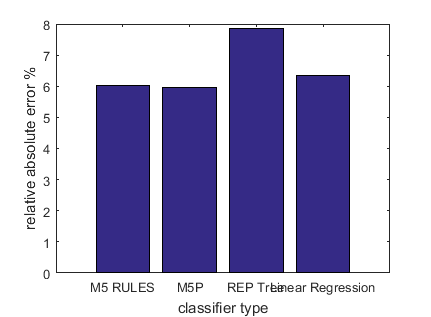
\includegraphics[width=\linewidth]{cluster-0-diff-classifier-relative-abs.png}
  \caption{cluster 0}
  \label{fig:cluster-0-predictors}
\end{minipage}%
\begin{minipage}{.5\textwidth}
  \centering
  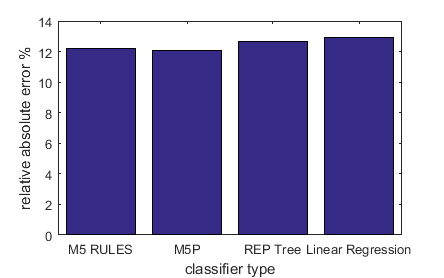
\includegraphics[width=\linewidth]{cluster-1-diff-classifier-relative-abs.png}
  \caption{cluster 1}
\label{fig:cluster-1-predictors}
\end{minipage}

\centering
\begin{minipage}{.5\textwidth}
  \centering
  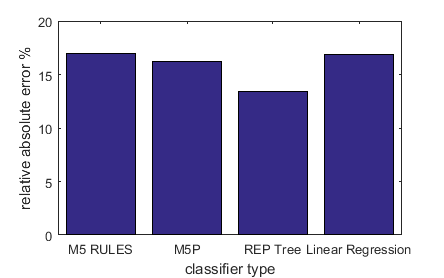
\includegraphics[width=\linewidth]{cluster-2-diff-classifier-relative-abs.png}
  \caption{cluster 2}
  \label{fig:cluster-2-predictors}
\end{minipage}%
\begin{minipage}{.5\textwidth}
  \centering
  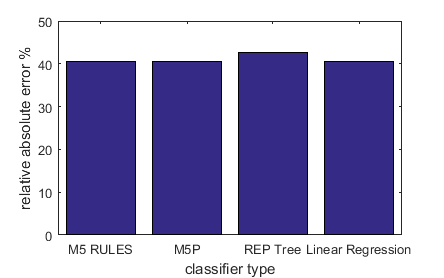
\includegraphics[width=\linewidth]{cluster-3-diff-classifier-relative-abs.png}
  \caption{cluster 3}
\label{fig:cluster-3-predictors}
\end{minipage}

\end{figure}
%% trial 1 end


\subsection{Comparison Among the Three Prediction Schemes}

Finally, all three demand prediction schems were tested with test set. From Figure \ref{fig:prediction-scheme-vs-error}, we can see that cluster based prediction mechanism performed almost as good as the mechanism individual prediction scheme, and it did much better than the default moving average prediction scheme. Individual prediction mechanism can be considered as a cluster based prediction mechanism with cluster size n. The cluster based mechanism used only 4 clusters, yet its performance was almost as same as the individual prediction mechanism. This suggests the importance of the cluster based prediction mechanism; it will need less amount of memory, the system is simple and generalized yet it produces quality prediction.

\begin{figure}[h!]
\centering
\begin{minipage}{.5\textwidth}
  \centering
  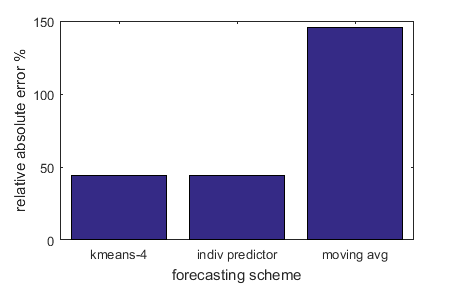
\includegraphics[width=\linewidth]{final-relative-abs-error.png}
  \caption{comparison among three prediction schemes}
  \label{fig:prediction-scheme-vs-error}
\end{minipage}
  
\end{figure}

\subsection{Model Accuracy and Training Set Size}
Figure \ref{fig:trainset-vs-error} shows the error of all three models with increasing training set size. It appears that the accuracy of the models does not change much with increased training set size. The reason behind this reason may be because the models were trained based on past tournament data. During a tournament the customer behavior remains unchanged, so adding more data may be redundant. 

\begin{figure}[h!]
  \centering
  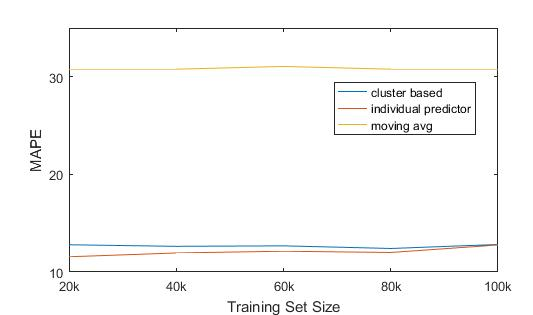
\includegraphics[width=\linewidth]{error-change-training-size.jpg}
  \caption{comparison among three prediction schemes}
  \label{fig:trainset-vs-error}
\end{figure}         % Chapter 5 Prediction Mechanism and result discussion
% chap6.tex (Conclusions and Future Work)

\chapter{Conclusions and Future Work}

\section{Significance of the Result}
This work showed that for each power type, a broker should use different demand forecasting mechanism. The work showed that for consumption type customers in the Power TAC simulation, the size of the cluster does not matter. The baseline with individual predictors can be considered as a mechanism with n customer, where n is the number of consumption customers. The proposed forecasting methodology was able to achieve almost similar demand forecasting mechanism using only 4 clusters. The above mentioned baseline has a serious fault, the demand predictors are hardcoded by the customer names. If during the simulation the name of a customer is changed, this mechanism will not work. On the other hand, the proposed mechanism can be trained on previous game logs and does not have the problem mentioned above.

\section{Future Work}

This work only deals with demand forecasting about the consumption customers. The proposed mechanism seems to be applicable for solar energy production customers with a slight change. For customer with irregular demand pattern such as customers with demand shifting capabilities and the electric vehicle customers, different technique of demand forecasting has to be figured out. 
         % Chapter 6
%% chap7.tex (Bogus chapter)

\chapter{Extra Chapter}

This is an extra chapter added into Patrick's thesis to illustrate
the use of figures and tables and the inclusion of a pdf file.

First the tables are shown as Table~\ref{smalltable} and
Table~\ref{smalltable2}. Then the
figure is shown in Figure~\ref{autom}.

\begin{table}
\begin{center}
\caption[A long caption]{A long caption.
In this table example, we have a very
long caption that does not fit on one line. The text of the
caption should line up on the left. The text inside the square
brackets will be included in the List of Tables.}
\label{smalltable}
\vspace{0.2in}
\begin{tabular}{|c|c|c|}\hline
2 & 3 & 300 \\ \hline
3 & 4 & 400 \\ \hline
4 & 5 & 500 \\ \hline
5 & 6 & 600 \\ \hline
\end{tabular}
\end{center}
\end{table}

\begin{table}
\begin{center}
\caption{Example of a table}
\label{smalltable2}
\vspace{0.2in}
\begin{tabular}{|c|c|c|}\hline
2 & 3 & 300 \\ \hline
3 & 4 & 400 \\ \hline
4 & 5 & 500 \\ \hline
5 & 6 & 600 \\ \hline
\end{tabular}
\end{center}
\end{table}

\begin{figure}
\begin{center}
\resizebox{\textwidth}{!}
  {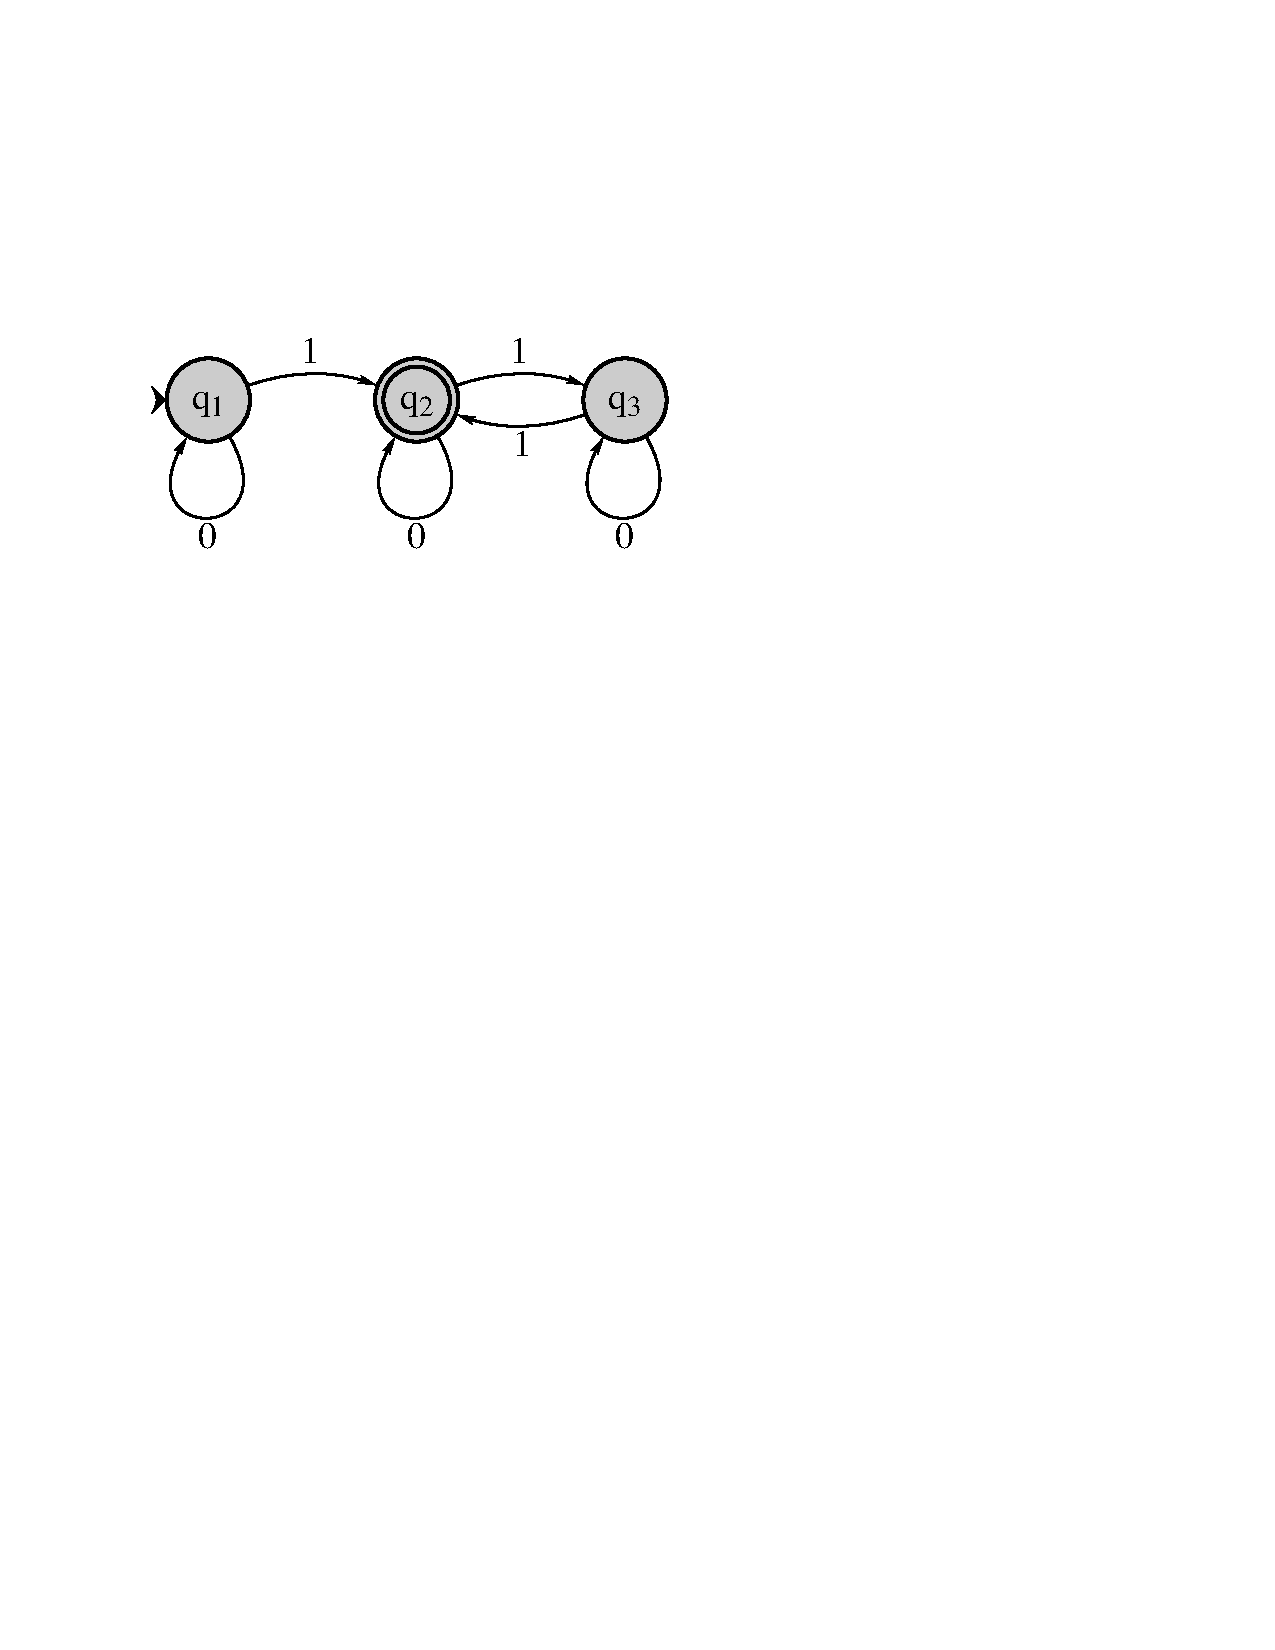
\includegraphics{automin1.pdf}}
\end{center}
\caption{A simple finite automaton}
\label{autom}
\end{figure}
         % Chapter 7, chap7.tex contains an
                        % example of figs and tables and inclusion of pdf.

%%%%%%%%%%%%%%%%%%%%
% Concluding Pages %
%%%%%%%%%%%%%%%%%%%%%%%%%%%%%%%%%%%%%%%%%%%%%%%%%%%%%%%%%%%%%%%%%%%%%%%%%%%%%%%%

% Bibliography or References, REQUIRED

% If using bibtex, create or modify the refs.bib file
% and use (uncomment) the following three lines.
%\bibliographystyle{plain}     %You may prefer \bibliographystyle{alpha}
%\addcontentsline{toc}{chapter}{\bibname}
\bibliography{refs}         
\bibliographystyle{plain}
% If using the ``thereference'' environment instead, modify the ref.tex file
% and use the following line
%% ref.tex {References}

\addcontentsline{toc}{chapter}{References}
\begin{thereferences}{99}

\bibitem{Cook1971}
S.~Cook,
 ``The complexity of theorem-proving procedures,''
 {\it Proceedings of the 3rd ACM Symposium on Theory of Computing},
 Shaker Heights, Ohio, 1971, pp.~151--158.

\bibitem{Garey1979}
M.~R.~Garey and D.~S.~Johnson,
 {\it Computers and Intractability: A Guide to the Theory of\/
 {\rm NP}-Completeness},
 W.~H.~Freeman, San Francisco, 1979.

\bibitem{Karp1972}
R.~Karp,
 ``Reducibility among combinatorial problems,''
 in: R.~Miller and J.~Thatcher (eds.),
 {\it Complexity of Computer Computations},
 Plenum Press, New York, 1972, pp.~85--103.

\bibitem{Kearfott1996}
R.~B.~Kearfott and V.~Kreinovich (eds.),
 {\it Applications of Interval Computations},
 Kluwer Academic Publishers, Norwell, MA, 1996.

\bibitem{Kreinovich1993}
V.~Kreinovich, A.~V.~Lakeyev and S.~I.~Noskov,
 ``Optimal solution of interval linear systems is intractable (NP-hard),''
 {\it Interval Computations},
 1993, No. 1, pp. 6--14.

\bibitem{Kreinovich1996a}
 V.~Kreinovich, A.~V.~Lakeyev and J.~Rohn ,
 ``Computational complexity of interval algebraic problems: some are feasible
 and some are computationally intractable: a survey,''
 in: G.~Alefeld and A.~Frommer (eds.),
 {\it Scientific Computing and Validated Numerics},
 Akademie-Verlag, Berlin, 1996, pp.~293--306.

\bibitem{Kreinovich1996b}
 V.~Kreinovich, A.~V.~Lakeyev, J.~Rohn and P.~Kahl,
 {\it Feasible? Intractable? On Computational Complexity of Data Processing
 and Interval Computations},
 Kluwer Academic Publishers, Norwell, MA, 1996 (to appear).

\bibitem{Kulisch1981}
U.~Kulisch and W.~L.~Miranker,
 {\it Computer Arithmetic in Theory and Practice},
 Academic Press, NY, 1981.

\bibitem{Lakeyev1995}
A.~V.~Lakeyev and V.~Kreinovich,
 ``If input intervals are small enough, then interval computations are almost
 always easy,''
 {\it Reliable Computing},
 Supplement (Extended Abstracts of APIC'95: International Workshop on 
 Applications of Interval Computations),
 1995, pp. 134--139.

\bibitem{Levin1973}
L.~Levin,
 ``Universal sequential search problems,''
 {\it Problems of Information Transmission},
 1973, Vol. 9, No. 3, pp. 265--266.

\bibitem{Moore1959}
R.~E.~Moore,
 ``Automatic error analysis in digital computation,''
 {\it Technical Report LMSD-48421},
 Lockheed Missiles and Space Co., Palo Alto, CA, January 1959.

\bibitem{Moore1966}
R.~E.~Moore,
 {\it Interval Analysis},
 Prentice Hall, Englewood Cliffs, NJ, 1966.

\bibitem{Neumaier1990}
A.~Neumaier,
 {\it Interval Methods for Systems of Equations},
 Cambridge University Press, Cambridge, 1990.

\bibitem{Rabinovich1995}
S.~G.~Rabinovich,
 {\it Measurement Errors: Theory and Practice},
 American Institute of Physics, NY, 1995.

\end{thereferences}


% If including appendices, uncomment the following lines,
% adding more includes if needed.
\StartAppendix
%\include{AppendixA}         % Example of how to include an appendix

% vitae.tex (Curriculum Vitae)

\addcontentsline{toc}{chapter}{Curriculum Vitae}
\chapter*{Curriculum Vitae}

Saiful Abu grew up in a small city called khulna in Bangladesh which was surrounded by rivers and forests. He is a first generation college graduate coming of a family with fish cultivation and agricultural background. He went to the most prestigious engineering school in nation, Bangladesh University of Engineering and Technology to study Bachelor of Science in Computer Science. He graduated from there in 2012. After working for a few years in the industry, he came to the University of Texas at El Paso in year 2014 during the fall. There he worked as Teaching assistant under the supervision of Dr. Olac Fuentes and Dr. Julio Urenda. He also worked as Research Assistant under the supervision of Dr. Christopher Kiekintveld. He graduated with a MS degree in Computer Science in Summer, 2016. 



\medskip

\noindent
Permanent address: 52, Jahidur Rahman Sarak

\noindent
\hspace{1.42in}
Khulna, Bangladesh.

\vfill

% The following is no longer needed when typed by the author.
%\noindent
%This thesis was typed by <name of typist>.


         % Curriculum Vitae      REQUIRED

%%%%%%%%%%%%%%%%%%%%%%%%%%%%%%%%%%%%%%%%%%%%%%%%%%%%%%%%%%%%%%%%%%%%%%%%%%%%%%%%


\end{document}
